\documentclass[a4paper,10pt]{article}

\usepackage[margin=1in]{geometry}

\usepackage[utf8]{inputenc}

\usepackage{graphicx}

\usepackage{float}

\usepackage{amssymb,amsmath}

\usepackage{colortbl}

\usepackage[table]{xcolor}

\usepackage[hidelinks]{hyperref}

\usepackage{rotating}

\makeatletter
\def\@maketitle{%
\newpage
%\null% DELETED
%\vskip 2em% DELETED
\vspace*{-1.0cm}
\begin{center}%
	\let \footnote \thanks
	{\LARGE \@title \par}%
	\vskip 1.5em%
	{\large
	\lineskip .5em%
	\begin{tabular}[t]{c}%
	\@author
	\end{tabular}\par}%
	\vskip 1em%
	{\large \@date}%
\end{center}%
\par
\vskip 1.5em}
\makeatother

\makeatletter
\newcommand{\thickhline}{%
	\noalign {\ifnum 0=`}\fi \hrule height 1pt
	\futurelet \reserved@a \@xhline
}
\newcolumntype{"}{@{\hskip\tabcolsep\vrule width 1pt\hskip\tabcolsep}}
\makeatother

\pdfinfo{%
  /Title    (Simple Pong Learner (SimPL): Utilizing a Genetic Algorithm to Tune the Weights of a Feed-Forward Neural Network)
  /Author   (Lettier)
  /Creator  (Lettier)
  /Producer (Lettier)
  /Subject  (machine learning)
  /Keywords (evolutionary genetic algorithm)
}

\title{Simple Pong Learner (SimPL): Utilizing a Genetic Algorithm to Tune the Weights of a Feed-Forward Neural Network}
\date{\today}
\author{Lettier}

\begin{document}

\maketitle

\begin{abstract}

The work presented here is motivated by the complex problem of tuning the parameters of a 3D physics engine via a genetic algorithm. A simpler, comparable domain was explored first, to provide a tractable basis for developing a robust genetic algorithm. A two-dimensional, asymmetric physics-based Pong clone was developed, called ``Simple Pong Learner'', or ``SimPL''.  The behavior of the pong-player's paddle is controlled via a feed-forward neural network consisting of 41 weights. The weights were tuned by a genetic algorithm. Five learning experiments were conducted in which training occurred over 100 generations. For comparison, two baseline experiments were also performed. Results show that the genetic algorithm produced paddles which performed better than the random baseline after 50 generations with even some results showing better than random after the first 10 generations. The next step is to apply lessons learned from developing the genetic algorithm used in SimPL to solve the harder problem of tuning the parameters of a 3D physics engine.

\end{abstract}

\section{Introduction}

\textbf{Sim}ple \textbf{P}ong \textbf{L}earner or SimPL is an asymmetric autonomous pong clone with one paddle and one ball. SimPL is comprised of web-based technologies: HTML5, JavaScript, CSS, AJAX, MySQL, and PHP. At the time of this writing, SimPL can be viewed at http://www.lettier.com/simpl/. The paddle in SimPL is controlled by a feed-forward neural network. The neural network's weights are tuned via a genetic algorithm. 

The focus for SimPL was to learn about and to cultivate a genetic algorithm capable of tuning parameters with respect to a fitness landscape thereby producing an optimum solution to a given parameter space. The genetic algorithm developed for SimPL will be used as a basis for a genetic algorithm needed to solve a harder problem of tuning a 3D physics engine. 

\section{Implementation}

\subsection{Arena}

The arena for SimPL resides in a browser window. Four transparent walls reside at the top, right, bottom, and left of the screen. The arena contains a ball and paddle with the paddle affixed to the far left of screen and the ball originating from the far right of the screen. See Figure \ref{fig:arena}.

\begin{figure}[H]  
  \centering
  
\includegraphics[width=.9\textwidth]{figures/arena.png}
  \caption{Here you see the SimPL arena containing the paddle and ball.}
  \label{fig:arena}
\end{figure}

\subsection{Ball}

The ball is a physics-based dynamic object. Its starting position and starting velocity magnitude are the same at the start of every round\footnote{A round is defined as the time from when the ball is launched from its starting position to either the time at which the ball leaves the left side of the arena or at the time in which the ball's velocity magnitude drops below $100$.}. Just before the beginning of a round, a random angle in the range $[135^\circ,225^\circ]$ is chosen as the ball's starting angle. See Figure \ref{fig:ball}. The ball's position is managed by the physics engine which responds to any collisions against the arena walls and/or the paddle.

\begin{figure}[H]  
  \centering
  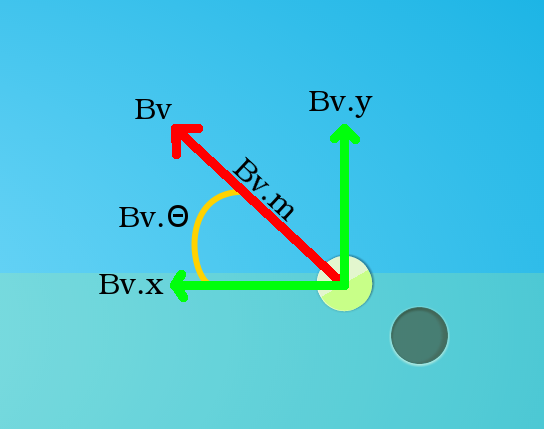
\includegraphics[width=.7\textwidth]{figures/ball.png}
  \caption{Here you see the ball's dynamic physics properties.}
  \label{fig:ball}
\end{figure}

If the ball collides with the left wall, the round is over. Otherwise, if the ball collides with the top, right, or bottom wall, the ball is bounced back into the arena via its angle-of-reflection based on its collision angle-of-incidence. Collisions with the paddle work in the same fashion where the ball is bounced back via its angle-of-reflection based on its collision angle-of-incidence. See Figure \ref{fig:angle}.

\begin{figure}[H]  
  \centering
  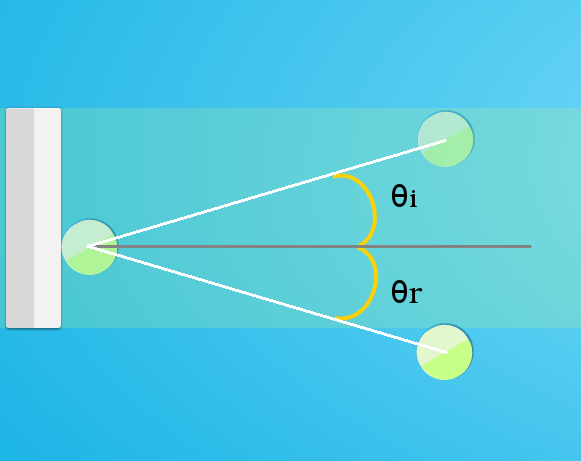
\includegraphics[width=.5\textwidth]{figures/angle.png}
  \caption{Here you see the ball's collision angle-of-incidence $\theta_i$ and its angle-of-reflection $\theta_r$.}
  \label{fig:angle}
\end{figure}

Each collision the ball makes reduces its velocity magnitude. Let $m$ denote the ball's velocity magnitude. The formula used is $m = m - (m * 50\%)$. Once the ball's velocity magnitude drops below $100$ the round is over.

\pagebreak

\subsection{Paddle}

The paddle is a physics-based dynamic object that has a fixed velocity angle of either $90^\circ$ or $270^\circ$. See Figure \ref{fig:paddle}. Its starting position as well as its starting velocity magnitude are the same at the start of every round. 

\begin{figure}[H]  
  \centering
  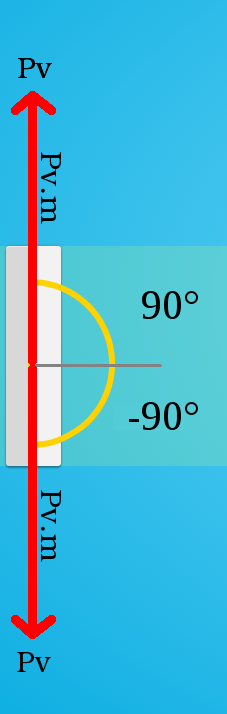
\includegraphics[width=.3\textwidth]{figures/paddle.png}
  \caption{Here you see the paddle's dynamic physics properties.}
  \label{fig:paddle}
\end{figure}

The paddle's direction and speed are regulated by the output of the neural network. The output of the neural network is in the range $[-1,1]$. A neural network output of $0$ results in the paddle not moving from its current position. A neural network output in the range of $(0,1]$ results in the paddle traveling up by some percentage of its starting velocity magnitude. A neural network output in the range of $[-1,0)$ results in the paddle traveling down by some percentage of its starting velocity magnitude. For example, say the neural network output is $0.68$ and let $m$ denote the paddle's velocity magnitude. The paddle's velocity angle would be set to $90^\circ$ and its velocity magnitude would be set to $m_{new}=0.68*m_{initial}$ where $m_{initial}$ is the paddle's starting velocity magnitude (specifically $1000 \ \frac{pixels}{second}$). Here the paddle can always travel as fast or faster than the ball given that the starting velocity magnitude of the paddle and ball are the same at the start of every round. However, while ball's velocity magnitude is reduced after every collision the ball makes, the paddle has the possibility of always traveling as fast as it could at the start of the round (albeit depending on the neural-network output). Thus, it is never the case that the paddle does not have the possibility of never reaching the ball in time during the duration of any round. In other words, it is never the case that the neural-network outputs the correct movement---given the paddle's and ball's states---but the paddle misses out on fitness it could have gained had it been traveling fast enough to reach the ball. The paddle can always reach the ball given the neural network output is correct given the paddle's and ball's states. Thus, at any time $t$ during any round $R_i$, the paddle's velocity magnitude is $0\leq m \leq 1000 \ \frac{pixels}{second}$ as $m = \left|[-1,1]\right| * m_{initial}$ where $\left|[-1,1]\right|$ is the absolute value of the neural-network's output range.    

Collisions can occur for the paddle between the top wall, the bottom wall, and the ball. Collision with either the top or bottom wall results in the paddle's top or bottom being placed just before the wall. Collision with the ball results in no change of movement for the paddle---the paddle merely continues moving as it was before the collision occurred with the ball.

\subsection{Physics Engine}

All dynamic and static objects are registered with the physics engine before the first round. Once every draw loop of the SimPL game, the physics engine tests for collisions between dynamic objects and other dynamic objects and between dynamic objects and static objects. Those dynamic objects that are found to be colliding with either another dynamic object and/or static object are flagged as such and their collisions are handled accordingly. For those dynamic objects that are not colliding, their positions are updated based on their velocity.

\subsection{Neural Network}

The neural network is a feed-forward neural network that contains one input layer consisting of six input nodes, one hidden layer consisting of 5 hidden nodes, and one output layer consisting of one output node \cite{neuralnetworks}. Each threshold input to the hidden nodes and the output node is included among the weights of the network and thus are optimized or tuned via the genetic algorithm. In total, there are 41 weights ($(6+1)*5+(5+1)*1=41$) contained in the network. See Figure \ref{fig:nn}. Thus, there are 41 genes per genome in the genetic algorithm's population. All output from the hidden nodes and the output node are run through a sigmoid, hyperbolic-tangent-activation function $\left ( tanh(x)=\frac{e^{2x}-1}{e^{2x}+1} \right )$ resulting in an output range of $[-1,1]$.

\begin{figure}[H]  
  \centering
  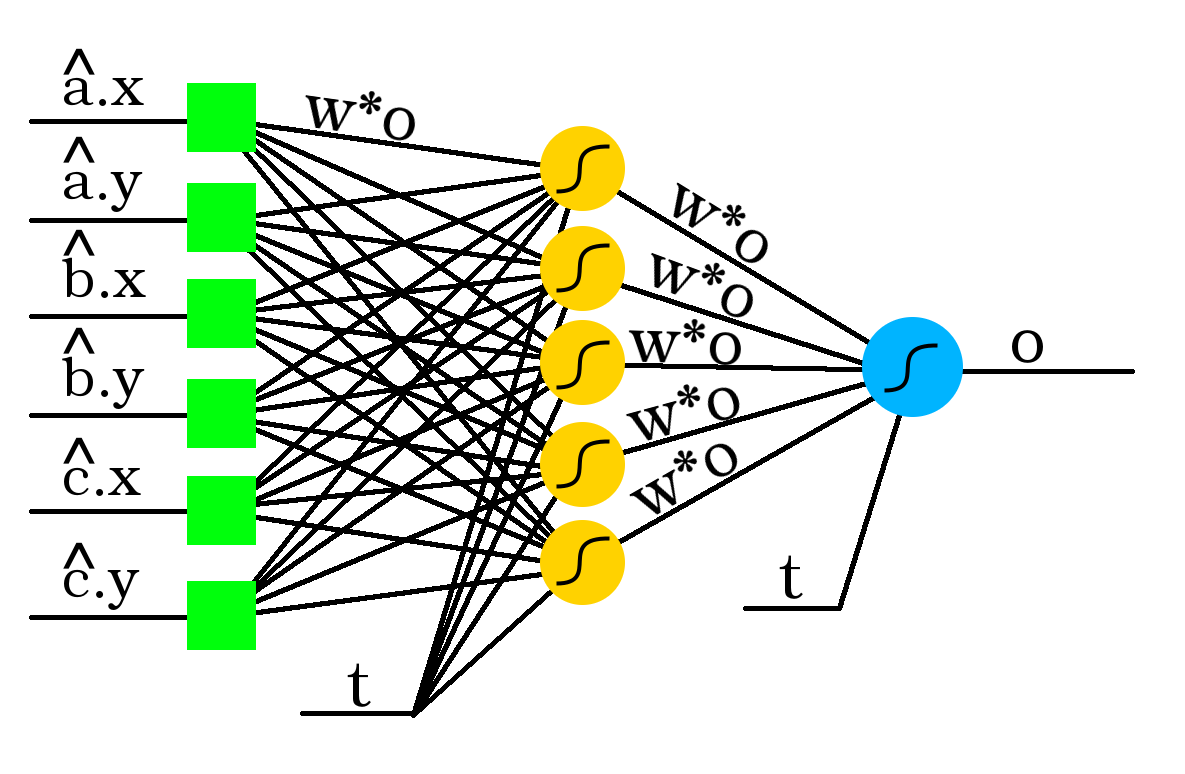
\includegraphics[width=1\textwidth]{figures/nn.png}
  \caption{Here you see the neural network as constructed in SimPL.}
  \label{fig:nn}
\end{figure}

Input to the neural network is normalized generating three unit vectors: from the ball's center to the paddle's center, the ball's velocity, and from the window's origin to the paddle's center. See Figure \ref{fig:unit_vectors}. These three unit vectors are broken down into their components resulting in six inputs to the neural network. See Figure \ref{fig:nn_input}. 

\begin{figure}[H]  
  \centering
  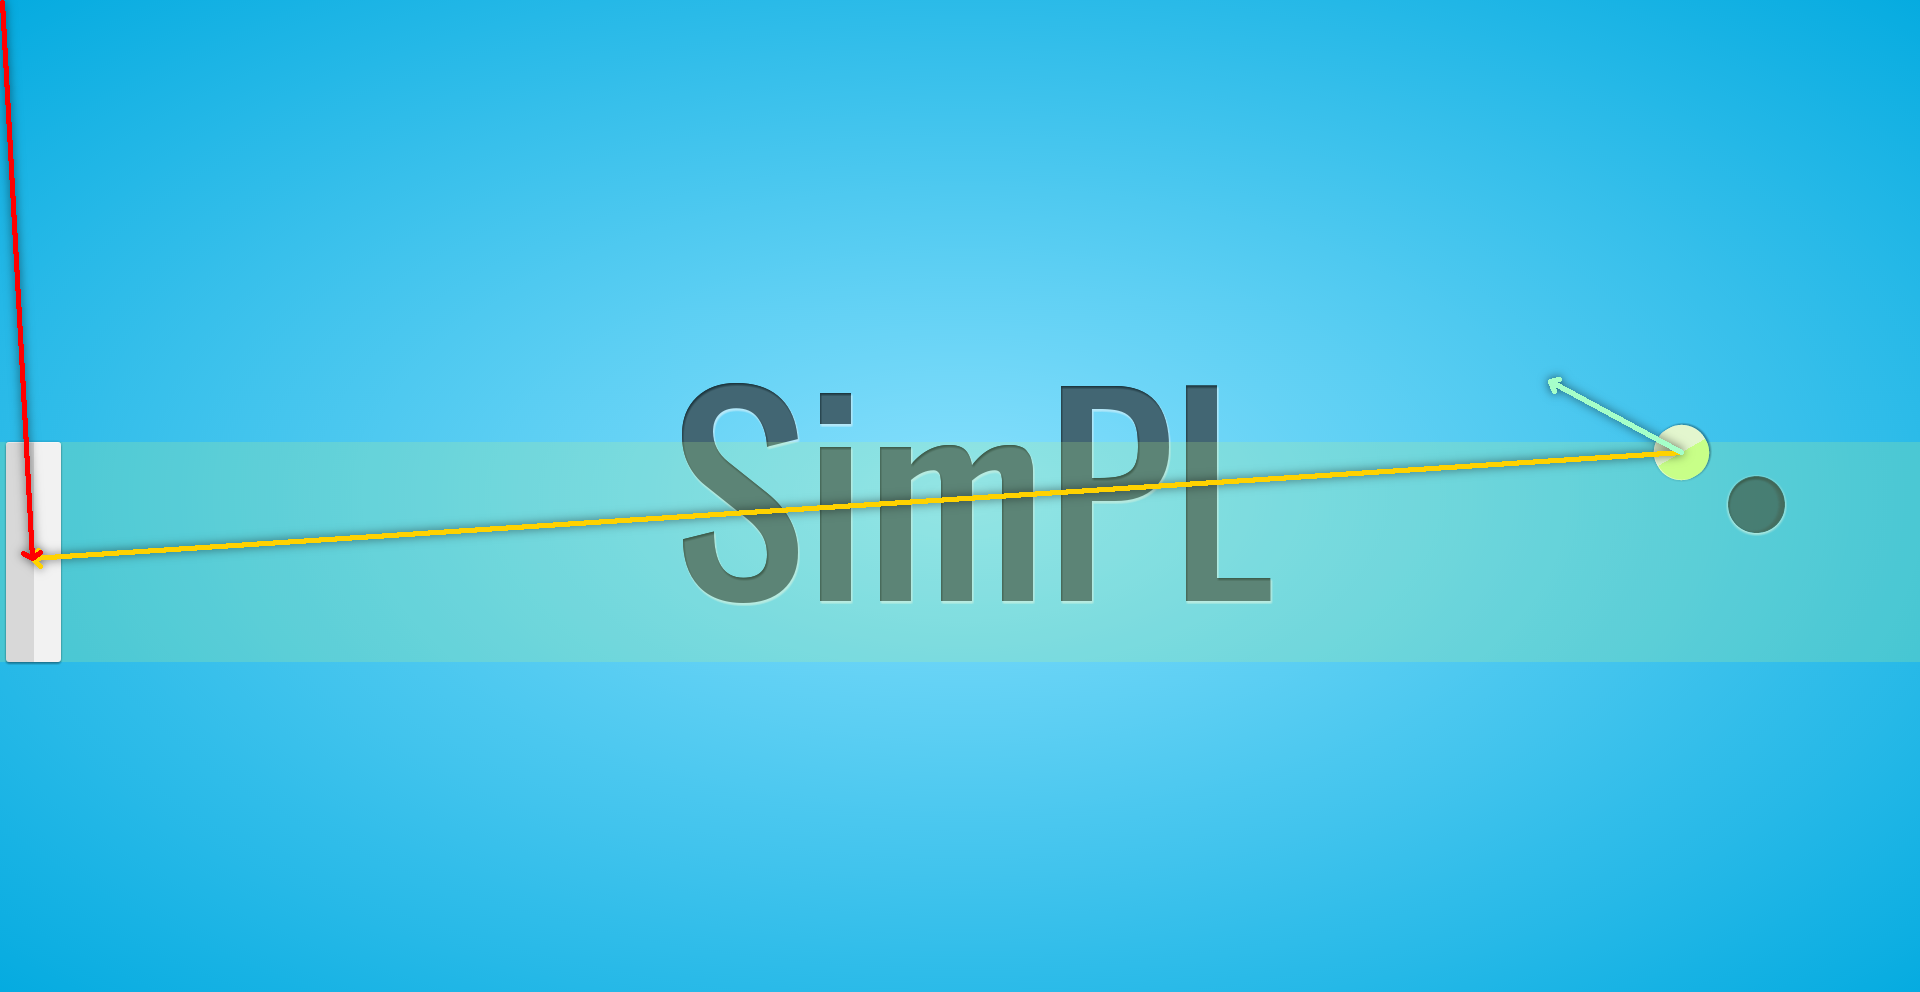
\includegraphics[width=1\textwidth]{figures/unit_vectors.png}
  \caption{Here you see the three input vectors to the neural network. Note that these vectors are normalized thereby turning them into unit vectors.}
  \label{fig:unit_vectors}
\end{figure}

\begin{figure}[H]  
  \centering
  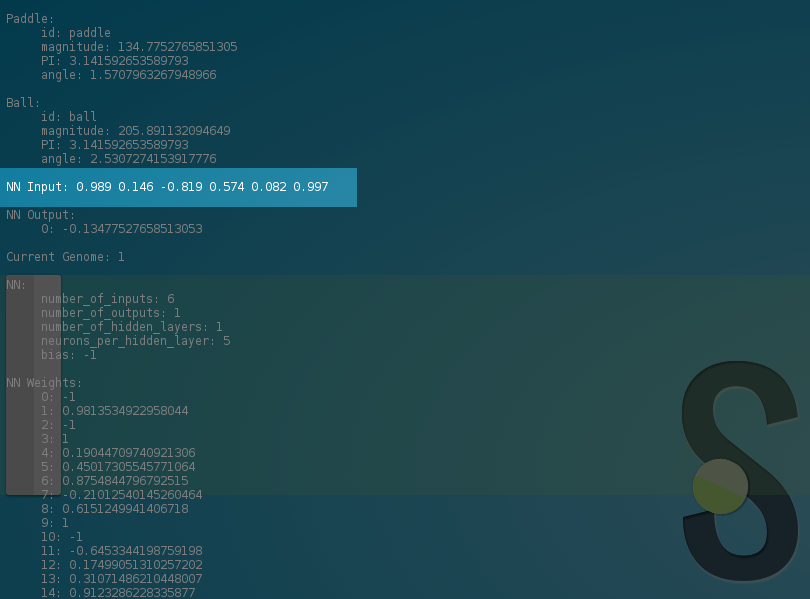
\includegraphics[width=.9\textwidth]{figures/nn_input.png}
  \caption{Here you see the normalized input to the neural network.}
  \label{fig:nn_input}
\end{figure}

\pagebreak

\subsection{Genetic Algorithm}

Instead of using back-propagation to train the weights of the neural network, a genetic algorithm is used to optimize or tune the weights of the neural network \cite{neuralnetworks}. The genetic algorithm consists of a population of genomes with each having a fitness property and an array of genes. For SimPL, the genes represent a solution of weights to be used in the neural network. Each genome is evaluated by a fitness function. As the genomes evolve over generations to produce fitter genomes, the neural network becomes increasingly accurate at outputting what the paddle should do (move up, stay still, or move down) based on the state of the ball and the paddle. 

The genetic algorithm contains four operators that work to produce fitter generations during the creation of a new population. The operators include: the elitism operator, the selection operator, the crossover operator, and the mutation operator. Initially, the genetic algorithm creates a random population of genomes. These initial genomes have zero fitness and a fixed number of genes. Each gene in every genome is given a random value sampled from a uniform distribution coinciding with some valid range. The genes are the input parameters to the mechanism the genetic algorithm is working to optimize. In the case of SimPL, the mechanism is the neural network and the parameters---of each genome---represent the 41 weights of the neural network. Each parameter has a valid range of $[-1,1]$. 

Once every genome in the population has been evaluated by the fitness function, the genetic algorithm constructs a new population from the previous generation. First, the elitism operator selects the $n$ fittest genomes from the old generation. These elite genomes are allowed to survive intact (however their fitnesses are reset to zero) and are placed into the new generation. Second, the genetic algorithm enters into a loop creating new genomes via the crossover operator and the mutation operator until an entirely new generation has been created. This new generation goes on to be evaluated as their predecessors were and the cycle repeats until some termination criteria is met. See Figure \ref{fig:ga}.

\begin{figure}[H]
\begin{equation*}
\boxed{
\begin{aligned}
Begin \ GA: & \\
&Generate \ population \ P_0. \\
& While \ not \ terminate: \\
& \quad\quad Evalute \ population \ P_i. \\
& \quad\quad Create \ empty \ populutation \ P_{i+1}. \\
& \quad\quad Sort \ P_i \ in \ non\!-\!decreasing \ order \ of \ fitness. \\
& \quad\quad Select \ n \ fittest \ from \ P_i \ and \ append \ to \ P_{i+1}. \\
& \quad\quad While \ |P_{i+1}| \ \leq \  population \ size: \\
& \quad\quad\quad\quad If \ perform \ crossover \ and \ mutation \ in \ sequence: \\
& \quad\quad\quad\quad\quad\quad g_1,g_2 \longleftarrow \ Select \ two \ genomes \ from \ P_i \ via \ roulette \ selection. \\
& \quad\quad\quad\quad\quad\quad /\!* \ Generate \ two \ of\! fspring \ via \ crossover. *\!/ \\
& \quad\quad\quad\quad\quad\quad o_1,o_2 \longleftarrow \ Crossover( g_1, g_2 ). \\
& \quad\quad\quad\quad\quad\quad /\!* \ Mutate \ crossover's \ of\!fspring \ and \\
& \quad\quad\quad\quad\quad\quad append \ to \ new \ population. \ *\!/ \\
& \quad\quad\quad\quad\quad\quad P_{i+1} \longleftarrow \ P_{i+1} + Mutate( o_1, o_2 ). \\
& \quad\quad\quad\quad Else: \\
& \quad\quad\quad\quad\quad\quad g_1,g_2 \longleftarrow \ Select \ two \ genomes \ from \ P_i \ via \ roulette \ selection. \\
& \quad\quad\quad\quad\quad\quad /\!* \ Generate \ two \ of\!fspring \ via \ crossover \\
& \quad\quad\quad\quad\quad\quad and \ append \ to \ new \ population. \ *\!/  \\
& \quad\quad\quad\quad\quad\quad P_{i+1} \longleftarrow \ P_{i+1} + Crossover( g_1, g_2 ). \\
& \quad\quad\quad\quad\quad\quad /\!* \ Mutate \ the \ two \ selected \ genomes \\
& \quad\quad\quad\quad\quad\quad and \ append \ to \ new \ population. \ *\!/  \\
& \quad\quad\quad\quad\quad\quad P_{i+1} \longleftarrow \ P_{i+1} + Mutate( g_1, g_2 ). \\
& \quad\quad P_{i} \longleftarrow P_{i+1}\\
\end{aligned}
}
\end{equation*}
\caption{Here you see the basic genetic algorithm.}
\label{fig:ga}
\end{figure}

\vspace{3mm}

The selection operator uses roulette selection where the probability of some genome being selected is proportional to their fitness. Roulette selection and roulette selection with rank fitness was experimented with as outlined later \cite{geneticalgorithm}. The crossover operator takes two selected genomes to produce offspring where the offspring have some combination of their parents' genes. SimPL uses one-point crossover throughout each experiment. To select the crossover point per crossover operation, the crossover operator samples a random integer from a uniform distribution ($crossoverPoint = X\!\sim\!U(0,n-1)$ where $n$ is the number of genes per genome). The mutation operator takes a selected genome and mutates its genes using various means. If the mutation scope is at the gene level, the mutation operator traverses through the genome's gene array where for each gene, the mutation operator samples a random integer from a uniform distribution ($X\!\sim\!U(0,1)$) and if this random integer $X$ is less than or equal to the mutation probability, the mutation operator mutates the gene value either via uniform mutation ($geneValue_i = X\!\sim\!U(0,1) * \varepsilon$) or Gaussian mutation ($geneValue_i = X\!\sim\!N(\mu,\sigma^2)$). If the mutation scope is at the genome level, the mutation operator samples a random integer from a uniform distribution ($X\sim U(0,1)$) and if this random integer $X$ is less than or equal to the mutation probability, the mutation operator mutates all of the genome's gene values one after the other via either uniform mutation ($geneValue_i = X\!\sim\!U(0,1) * \varepsilon$) or Gaussian mutation ($geneValue_i = X\!\sim\!N(\mu,\sigma^2)$). These means of mutation were experimented with as outlined later. Crossover and mutation can be carried out in sequence or can be done separately with one operator not interfering the other operator's offspring. This was experimented with as outlined later.

Crossover and mutation are not guaranteed to always occur as the genetic algorithm produces new genomes from the old genomes. Rather, crossover and mutation occur based on some probability. If the crossover and mutation probabilities are both set to $1$ then they always occur. Before the genetic algorithm is initialized, the crossover and mutation probabilities are set \cite{self_adapt}. These initial crossover and mutation probability values can be arbitrary or can be based on some a-priori knowledge of the fitness landscape. The probabilities can change over time or can remain static throughout the run of the genetic algorithm. Different static settings and self-adaptation of the probabilities were experimented with as outlined later. 

The fitness function evaluates each genome in the current population based on some fitness criteria. The fitness criteria coincides with finding the optimum solution to the parameter space of the mechanism the genetic algorithm is producing fitter and fitter solutions to. For SimPL, the parameter space is the weights of the neural network. Each genome represents a solution or point in the weights space. An optimal solution in the weights space will make the neural network always give a correct output as to what movement the paddle must make based on the ball's and the paddle's current states. This will result in the paddle always following the ball or in other words, the paddle will never let the ball leave the left side of the screen. Thus the fitness criteria for SimPL could include how much or how well the paddle follows the ball and/or how many times the paddle hits the ball. Different fitness criteria were experimented with as outlined later. 

% GA loop
% crossover
% mutation
% observed rates
% perturbation
% Gaussian mutation
% whole versus gene-by-gene mutation
% sequential operators versus separate
% self-adaptation via tracking progress
% partial credit fitness

\subsection{Database Manager}

A database manager interfaces with a remote MySQL server either asynchronously or synchronously. Experiment data is recorded in the MySQL database as the experiment is carried out. Additionally, each generation produced by the genetic algorithm is logged to the database. Upon visiting the SimPL site, the last generation produced can be loaded into the genetic algorithm thereby allowing the simulation to pick up where it left off last.  

\section{Platform}

The browser window size has a significant influence over the fitnesses of the genomes being evaluated. While the arena fits to whatever size the browser window is, the size of the paddle and the ball do not directly change in proportion to the window size. Thus, a small browser window gives the paddle less screen real estate to cover in comparison to a large browser window. For example, imagine a browser window size with a height as large as the paddle's height. Here the paddle can never move---it always follows the ball and always hits the ball. Thus, the resulting fitnesses observed would be erroneously high. Therefore, all experiments were run using the same browser window size. 

%it is important to note what platform SimPL was run on when discussing experimental results---especially when comparing experimental results with one another. Care was taken to run experiments on the same platform when the experiments would be directly compared to one another. 

%The laptop's browser window size is $\sim70\%$ the size of the desktop browser window size (see Figure \ref{fig:platform_sizes}) and thus higher fitnesses are observed when comparing identical runs of the genetic algorithm performed on the laptop versus the desktop. On the desktop the paddle has $992-220=772$ pixels to traverse while on the laptop the paddle has $681-200=481$ pixels to traverse.

%\begin{figure}[H]  
%  \centering
%  
\includegraphics[width=.666\textwidth]{figures/platform_sizes.png}
%  \caption{Here you see the laptop screen superimposed onto the desktop screen.}
%  \label{fig:platform_sizes}
%\end{figure}

%1526.3410497 / 2161.125632628  = 0.706271318

%\subsection{Desktop}

%Google Chrome version number 26.0.1410.63 was used on the desktop. Screen resolution was $1920\times1080$. Browser window size (both reported and actual) was 1920 pixels wide by 992 pixels tall. Paddle size reported (by the browser) was 50 pixels wide by 200 pixels tall but the actual size was 55 pixels wide by 220 pixels tall. Ball size reported (by the browser) was 50 pixels wide by 50 pixels tall but the actual size was 57 pixels wide by 57 pixels tall.

%\subsection{Laptop}
Experiments were run on a Lenovo Z580 Ideapad laptop running 64-bit Fedora 18 and was equipped with an Intel Core i5 CPU running at 2.5 GHz and 7.7 GiBs of memory. Google Chrome version number 30.0.1599.114 was used on the laptop. Screen resolution was $1366\times768$. Browser window size (both reported and actual) was 1366 pixels wide by 681 pixels tall. Paddle size reported (by the browser) was 50 pixels wide by 200 pixels tall and the actual size was the same. Ball size reported (by the browser) was 50 pixels wide by 50 pixels tall and the actual size was the same. The paddle had $681-200=481$ pixels of available screen-space to traverse.  

\section{Experimental Designs}

Each SimPL experimental design (with the exception of experiments six and seven) was constructed in such a way as to focus on a set of one or more facets to the genetic algorithm. See Table \ref{tab:exps}. With each progressive experiment, the facets not focused on were kept the same from the previous experiment. The goal was to create a genetic algorithm that would eventually---with efficiency---produce the optimal set of neural-network weights needed in order to generate a paddle that performs as well as the performance-standard paddle constructed in experiment six. Ultimately, the performance of any paddle in SimPL is how long it keeps the ball-in-play before the termination of any round.       

Experiments one and two revolved around the fitness function, the selection operator, and the static crossover and static mutation properties of the genetic algorithm. Experiments three, four, and five revolved around the self-adaptation of the crossover and mutation probabilities and whether allowing the mutation operator to disrupt the offspring, produced by the crossover operator, degraded the performance of the genetic algorithm. Experiment six revolved around constructing a paddle as an optimal-performance standard by which any other paddle could be measured by. Finally, experiment seven revolved around constructing a randomly behaving paddle thereby producing a performance lower bound.

For each experiment, the genetic algorithm was run for 100 generations where for each generation, the population's average fitness was recorded. Once every 10th generation, the current population's top performing genome was saved. After the run of the genetic algorithm was over, the saved top-performers were run in a tournament. This tournament consisted of running each top-performer for five rounds where for each top performer, the time in seconds they kept the ball-in-play per round was recorded. Once an every-10th-generation-top-performer was done with their five rounds, the average of their ball-in-play time per round was calculated and recorded.   

\renewcommand*\arraystretch{1.5}

\begin{sidewaystable}
\begin{table}[H]
%\hskip-1.7cm
%\footnotesize
\centering
    \begin{tabular}{ | >{\columncolor{lightgray}} r"c|c"c|c|c"c| } \hline
    \rowcolor{lightgray} \textbf{GA Parameters $\times$ Experiment} & \textit{One} & \textit{Two} & \textit{Three} & \textit{Four} & \textit{Five} & \textit{Six \& Seven}  \\ \thickhline 
    \textit{Population Size} & 10 & 10 & 10 & 10 & 10 & 10 \\ \hline 
    \textit{Fitness Function Type} & \cellcolor{blue!25} Partial/Full & \cellcolor{blue!25} Full & Full & Full & Full & Full \\ \hline
    \textit{Number of Elite Offspring} & 2  & 2 & 2 & 2 & 2 & 10  \\ \hline
    \textit{Roulette Selection - Actual Fitness} & True & \cellcolor{blue!25} False  & False & False & False & N/A \\ \hline
    \textit{Roulette Selection - Rank Fitness} & False & \cellcolor{blue!25} True & True & True & True & N/A \\ \hline
    \textit{Sequential Crossover \& Mutation} & True & True & \cellcolor{blue!25} False & False & \cellcolor{blue!25} True & N/A \\ \hline
    %\textit{Parents Survive} & True & True & \cellcolor{blue!25} False & False & False & N/A \\ \hline
    \textit{Self-adaptation} & False & False & \cellcolor{blue!25} True & \cellcolor{blue!25} False & False &  N/A \\ \hline
    \textit{Crossover Type} & One-point & One-point & One-point & One-point & One-point & N/A \\ \hline
    \textit{Crossover Probability }& 0.7 & \cellcolor{blue!25} 0.8 & \cellcolor{blue!25} 0.5 & \cellcolor{blue!25} 0.7816 & 0.7816  & N/A \\ \hline
    \textit{Mutation Type} & Uniform & \cellcolor{blue!25} Gaussian & Gaussian & Gaussian & Gaussian &  N/A \\ \hline
    \textit{Mutation Scope} & Gene & Gene & \cellcolor{blue!25} Genome & Genome & \cellcolor{blue!25} Gene & N/A \\ \hline
    \textit{Mutation Probability } & 0.1 & \cellcolor{blue!25} $\left(\frac{1}{n}\right)=\left(\frac{1}{41}\right) \approx 0.0244$ & \cellcolor{blue!25} 0.5 & \cellcolor{blue!25} 0.2184 & 0.2184 & N/A \\ \hline
    \textit{Mutation Step} & $X\sim U(0,1) * 0.3$ & \cellcolor{blue!25} $X\sim N(\mu,\sigma^2)$ & $X\sim N(\mu,\sigma^2)$ & $X\sim N(\mu,\sigma^2)$ & $X\sim (\mu,\sigma^2)$ & N/A \\ \hline
    \textit{Mutation Step} $\mu$ & N/A & \cellcolor{blue!25} Gene Value & Gene Value  & Gene Value  & Gene Value & N/A \\ \hline
    \textit{Mutation Step} $\sigma$ & N/A & \cellcolor{blue!25} 0.5 & \cellcolor{blue!25} $M_{Prob.}$ & $M_{Prob.}$ & $M_{Prob.}$ & N/A \\ \hline
    \end{tabular}
\caption{Here you see the genetic algorithm parameters used per experiment. The highlighted cells indicate the experimental variables per experiment. Experiment six and seven are included in the table for completeness but no evolution ever took place.}\label{tab:exps}
%\normalsize
\end{table}
\end{sidewaystable}

\subsection{Experiment one: use of a full and partial credit granting fitness function.}

Experiment one centered around the use of a fitness function that would give full and partial credit based on the behavior of the neural network and thus the paddle. The genetic algorithm parameters used are listed in Table \ref{tab:exp1}.

During each generation of the genetic algorithm, each genome from the population was allowed to run one round until the round terminated either due to the ball leaving the left side of the screen or the ball's velocity magnitude dropping below $100$. Note that during the round, the paddle's movement (in relation to the ball's movement) was tracked via an array as well as how many times the paddle hit the ball during the round. Once the round terminated, the genome was evaluated by the fitness function. During evaluation, if the genome's phenotype (the paddle's observable characteristics) followed the ball (from one draw loop to next) it would be given a positive partial fitness credit of $0.1$ every time it followed the ball. If the phenotype managed to collide with the ball, the genome was given a full fitness credit of $1$ every time it hit the ball. However, if the phenotype moved away from the ball (from one draw loop to the next), it was given a negative partial fitness credit of $-0.1$ every time it moved away from the ball. Lastly, if the phenotype didn't move at all (while the ball moved from one draw loop to the next) it was given $0$ fitness every time it did not move. At the end of the fitness function, all of these partial and full fitness credits were summed giving the currently-being-evaluated genome its total fitness. If the total summed fitness was less than zero, the total summed fitness was set to zero. That is, no genome's fitness---after having been evaluated by the fitness function at the end of its round---was ever negative. 

To facilitate tracking the paddle's movements in relation to the ball's movements (during the round), the absolute difference in heights between the paddle's center and the ball's center were recorded every draw loop into an array. Once the genome was ready to be evaluated, this array of differences was analyzed linearly in pairs, that is, $A[i]$ was compared with $A[i+1]$. If $A[i]>A[i+1]$ this indicated that the paddle's center was moving closer to the ball's center and thus the genome was awarded a positive partial credit fitness. If $A[i]<A[i+1]$ this indicated that the paddle's center was moving away from the ball's center and thus the genome was awarded a negative partial credit fitness. If $A[i]=A[i+1]$ this indicated that the paddle's center was neither moving toward nor away from the ball's center and thus the genome was awarded $0$ fitness. A special case for $A[i]=A[i+1]$ was that if $A[i]=0$ and thus $A[i+1]=0$ as well, the paddle was awarded a positive partial fitness as the paddle's center was dead center with the ball's center and therefore the paddle was directly in the path of the ball which is ultimately the goal---that is, the paddle should always match its center with the ball's center thereby always preventing the ball from leaving the arena.

The hypothesis for using a full and partial fitness credit schema was that every new generation produced would have genomes that at least performed somewhat better than their predecessors at the optimal behaviors. Those optimal behaviors are following the ball and hitting the ball. Originally, only hitting the ball was going to be the fitness criteria. However, early generations may never hit the ball and thus would have zero fitness. Genomes that at least followed the ball could have been erroneously discarded due to having zero fitness. By giving partial credit for at least following the ball, it was hypothesized that it would seed early generations with promising genomes or rather promising solutions to the parameter space. Picture a classroom of students taking a test. Upon evaluation, it is either all or nothing credit per question and no student finds the solution to any problem. In other words, every student received a zero. This would give the teacher no information as to the quality of the students at least in terms of comparing them to one another. However, if partial credit is given for getting part of the solution correct, then this would give at least some information as to who performed well among the students. In other words, it was hypothesized that by using a finer grained fitness function, there would be some information gained as to the fitness of one genome compared to another (aiding elitism and the selection process) versus no information gained using only a coarsely grained fitness function resulting in every genome having a fitness of zero after being evaluated.

\begin{table}[H]
\centering
\footnotesize
\begin{tabular}{ |>{\columncolor[gray]{0.8}} l | l| }
\hline
Population Size                                                      & 10                                                        \\ \hline
Number of Elite Offspring                                            & 2                                                         \\ \hline
Roulette Selection using Actual Fitness                              & True                                                      \\ \hline
Roulette Selection using Rank Fitness                                & False                                                     \\ \hline
Crossover Probability                                                & 0.7                                                       \\ \hline
Crossover Type                                                       & One Point Crossover                                       \\ \hline
Mutation Probability                                                 & 0.1                                                       \\ \hline
Mutation Scope                                                       & Gene Level                                                \\ \hline
Mutation Step                                                        & $X\sim U[-1,1] \ *$ Max-Perturbation                      \\ \hline
Max-Perturbation                                                     & 0.3                                                       \\ \hline
Sequential Crossover and Mutation                                    & True                                                      \\ \hline
%Offspring not Crossed/Mutated Allowed in New Generation             & True                                                      \\ \hline
Fitness Function                                                     & Partial/Full                                              \\ \hline
Fitness Credit for Hitting the Ball                                  & 1.0                                                       \\ \hline
Fitness Credit for Following the Ball                                & 0.1                                                       \\ \hline
Fitness Credit for Matching the Ball's Center Y-coordinate           & 0.1                                                       \\ \hline
Fitness Credit for not Following the Ball                            & -0.1                                                      \\ \hline
\end{tabular}
\caption{Here you see the genetic algorithm parameters for experiment one.}
\label{tab:exp1}
\end{table}

\subsection{Experiment two: use of a simplified fitness function, use of rank fitness in selection, higher crossover probability, mutation probability based on the number of genes per genome, and a Gaussian distribution sample mutation step.}

% Talk about wide gaps of fitness. Giving poor performers at least some chance of being selected for crossover and mutation. Keeping the population diverse and avoiding early convergence due to the top performers just swapping the same genes over and over after x generations.

Experiment two had a simplified fitness function, used a genome's rank fitness during selection, increased the crossover probability, based the mutation probability on the number of genes per genome, and used Gaussian distribution sampling as the mutation step. The genetic algorithm parameters used are listed in Table \ref{tab:exp2}.

Going from awarding full and partial credit fitness based on two behaviors to only awarding a fitness credit of $1$ if the paddle was in the path of the ball per every draw loop, the fitness function was simplified. Here the paddle doesn't necessarily have to be dead center to the ball but rather the paddle's top must be at or above the ball's top while at the same time the paddle's bottom has to be at or below the ball's bottom. See Figure \ref{fig:simple_fit_func}. The reasoning behind this was that if the paddle were to always be in the path of the ball then it would always hit the ball and thus the paddle would never let the ball leave the arena or in other words the paddle would exhibit the optimum desired behavior. Therefore, this fitness function correctly evaluates the paddle's (or rather the genome phenotype's) behavior in relation to ball's movement throughout any round.

\begin{figure}[H]  
  \centering
  
\includegraphics[width=.45\textwidth]{figures/simple_fit_func.png}
  \caption{Here you see the simplified fitness function graphically where the paddle on the left is gaining fitness (as indicated by the green-hued bar) while the paddle on the right is gaining no fitness (as indicated by the purple-hued bar).}
  \label{fig:simple_fit_func}
\end{figure}

Instead of using the actual fitness of any particular genome in the population to determine its probability of being selected during the roulette wheel selection process, a genome's rank fitness was used to determine its probability of being selected \cite{geneticalgorithm}. It was observed during early runs of the genetic algorithm that after evaluation the population had wide gaps of fitness. The genomes with zero or relatively low fitness had absolutely little to no chance of being selected for crossover and mutation while the genomes with a relatively high fitness had a high chance of being selected for crossover and mutation. These early top performers were continuously selected, crossed, and mutated generation after generation. Population diversity dwindled thereby causing the population to converge too early (due to an ever narrowing search of the fitness landscape) resulting in poor performance on behalf of the genetic algorithm. Thus it was hypothesized that by using rank fitness instead of actual fitness to determine a genome's probability of being selected, population diversity would remain sufficient generation after generation thereby avoiding early convergence. 

Rank fitness is a genome's fitness according to their index in the population after the population is sorted in increasing order of fitness \cite{genselect}. After sorting the population, genome one is given a fitness of one, genome two is given a fitness of two and so on and so forth until genome $n$ is given a fitness of $n$ or rather the population size. See Figure \ref{fig:roulette}. Now all genomes have a better chance of being selected to undergo crossover and/or mutation thereby keeping the population diversity high and thus keeping the search scope of the fitness landscape large resulting in better performance of the genetic algorithm.   

\begin{figure}[H]  
  \centering
  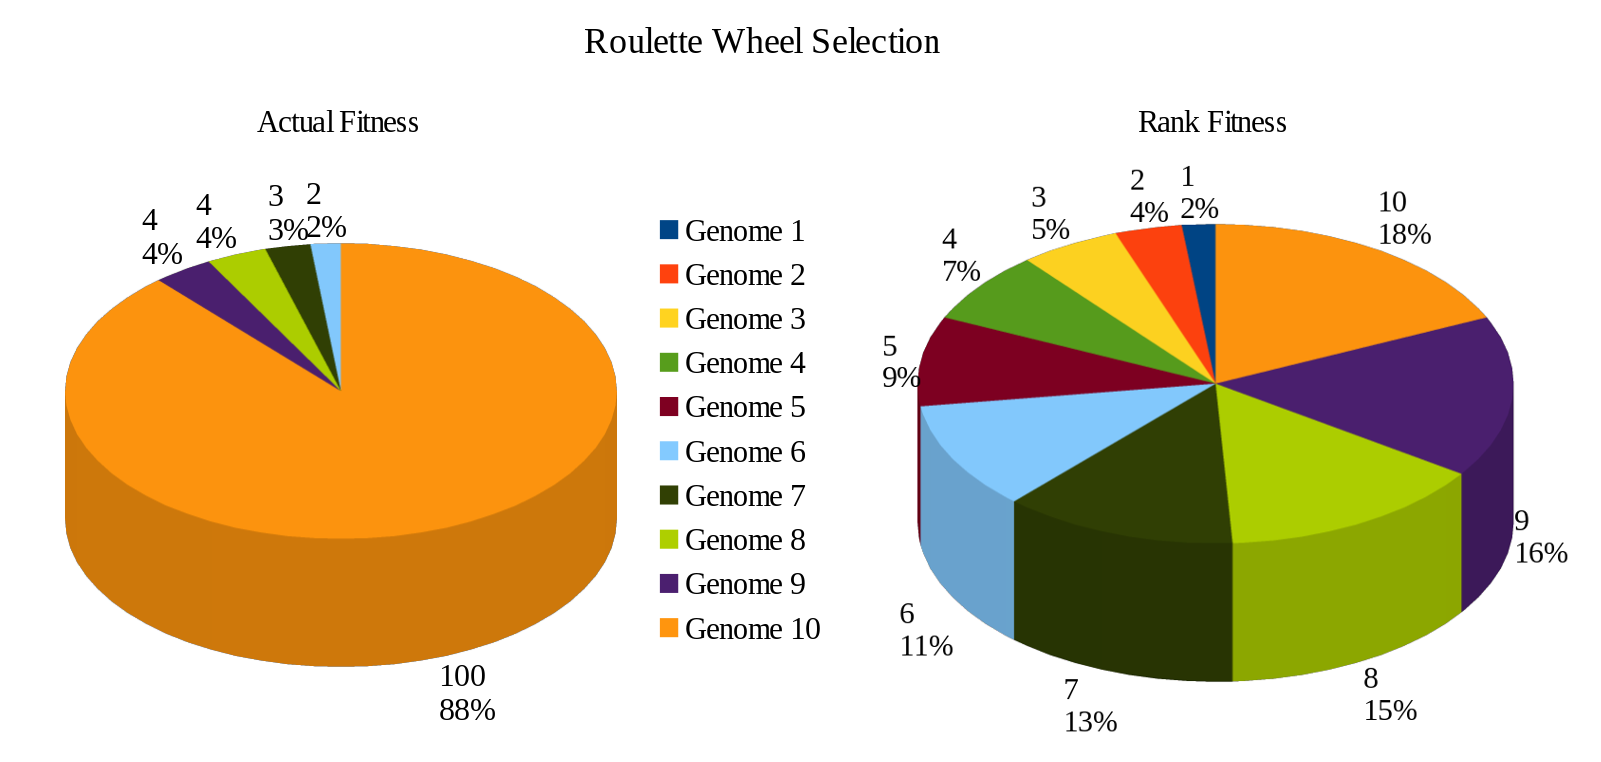
\includegraphics[width=.9\textwidth]{figures/roulette.png}
  \caption{Here you see roulette selection using actual fitness versus rank fitness for a population of 10 genomes. On the left, the integers are the genomes' actual fitness and the percentages are their probabilities of being selected. On the right, the integers are the genomes' rank fitness and the percentages are the genomes' probabilities of being selected. Observe that Genome 10 no longer dominates the wheel when using its rank fitness ($10$) versus using its actual fitness ($100)$.}
  \label{fig:roulette}
\end{figure}

Crossover probability was increased from $0.7$ to $0.8$. This of course would result in more observed crossovers being generated as new populations were created. Since crossover produces an offspring solution  somewhere between its parents in the fitness landscape, it was hypothesized that by increasing the crossover probability the local search capability of the genetic algorithm would also increase.

Based on empirical studies performed by others, setting the mutation probability to $\frac{1}{n}$---where $n$ is the number of genes per genome---is a sufficient enough amount of random search to allow the genetic algorithm to escape local maxima in the fitness landscape \cite{predictive_models}. The reasoning behind $\frac{1}{n}$ is that per mutation on a gene-by-gene basis, only one gene is mutated on average. In addition to changing the mutation probability, the mutation step was changed from adding and/or subtracting a percentage of a maximum perturbation parameter value to and/or from the gene value to sampling a value from a Gaussian distribution where the distribution $N(\mu,\sigma^2)$ is defined by the mean $\mu$ being the gene's current value before mutation and the standard deviation $\sigma$ being one fourth the valid range of the gene/parameter $\left(\frac{1-(-1)}{4}=0.5 \right)$. Here the standard deviation $\sigma$ is one fourth the range and thus most of the sampled values will be within two standard deviations of the mean $\mu$ or rather the gene value. Any sampled gene value that was outside the valid range of $[-1,1]$ was clipped to the valid range. Note that by going with this new mutation step schema, the maximum perturbation parameter to the genetic algorithm could be removed thereby lessening the amount of parameters---to the genetic algorithm---that need to be evaluated. 

\begin{table}[H]
\centering
\footnotesize
\begin{tabular}{ |>{\columncolor[gray]{0.8}} l | l| }
\hline
Population Size                                                      & 10                                                                \\ \hline
Number of Elite Offspring                                            & 2                                                                 \\ \hline
Roulette Selection using Actual Fitness                              & False                                                             \\ \hline
Roulette Selection using Rank Fitness                                & True                                                              \\ \hline
Crossover Probability                                                & 0.8                                                               \\ \hline
Crossover Type                                                       & One Point Crossover                                               \\ \hline
Mutation Probability                                                 & $\frac{1}{n \ genes}=\frac{1}{41} = 0.024390244$                  \\ \hline
Mutation Scope                                                       & Gene Level                                                        \\ \hline
Mutation Step                                                        & $X\sim N(\mu,\sigma^2)$                                           \\ \hline
Mutation Step $\mu$                                                  & Gene Value                                                        \\ \hline
Mutation Step $\sigma$                                               & $0.5$                                                             \\ \hline
Max Perturbation                                                     & N/A                                                       	       \\ \hline
Sequential Crossover and Mutation                                    & True                                                      	       \\ \hline
%Offspring not Crossed/Mutated Allowed in New Generation             & True                                                     	       \\ \hline
Fitness Function                                                     & Full                                                              \\ \hline
Fitness Credit for Staying in the Path of the Ball                   & 1.0                                                      	       \\ \hline
Fitness Credit for not Staying in the Path of the Ball               & 0.0                                                      	       \\ \hline
\end{tabular}
\caption{Here you see the genetic algorithm parameters for experiment two.}
\label{tab:exp2}
\end{table}

\subsection{Experiment three: self-adaptation of crossover and mutation probabilities with the crossover and mutation operators working in parallel.}

Experiment three involved self-adaptation of the crossover and mutation probabilities. The genetic algorithm parameters used are listed in Table \ref{tab:exp3}.

As outlined in \cite{self_adapt}, the crossover and mutation probabilities self-adapt based on the crossover and mutation operators' ability to produce fitter genomes from one generation to the next. To facilitate the self-adaptation, the crossover and mutation operators' viability to produce fitter and fitter offspring needed to be tracked from one generation to another. As the operators were being evaluated on their own accord, they were not allowed to interfere with each others' offspring and thus they were not run in sequence but rather were run in parallel. With each new generation produced, elite offspring were marked accordingly as well as offspring produced by crossover and offspring produced by mutation. For those offspring that were created by crossover, their parents' weighted-mean fitness was annotated along with their offspring. Annotated meaning it was recorded in the offspring's data structure later being used to calculate the crossover operator's progress. This weighted-mean fitness was calculated based on the crossover point which determines what percentage of genes came come from parent one and what percentage of genes came from parent two. For example, let there be 41 genes per genome and let the crossover point be gene 10. Thus, offspring one received 10 genes from parent one and received 31 genes from parent two while offspring two received 10 genes from parent two and received 31 genes from parent one. Therefore, offspring one's weighted-mean parent fitness would be calculated as $\overline{PF} = \left ( PF_1 * \frac{10}{41} \right ) + \left (PF_2 * \frac{(41-10)}{41} \right)$ where $\overline{PF}$ is the weighted-mean parent fitness while offspring two's weighted-mean parent fitness would be calculated as $\overline{PF} = \left ( PF_2 * \frac{10}{41} \right ) + \left (PF_1 * \frac{(41-10)}{41} \right)$. For those offspring created via mutation, their parent fitness was whatever the fitness was of the pre-mutated genome. 

With the genomes marked as to how they were created and their parent fitness annotated, now when it came time to produce a new population, each operators' ability to produce fitter offspring could be tracked and calculated. Once a population was evaluated, all genomes created by crossover were used to calculate the average crossover progress and all genomes created by mutation were used to calculate the average mutation progress. If the crossover progress average was greater than the mutation progress average then the crossover probability would be adjusted up and the mutation probability would be adjusted down. Alternatively, if the crossover progress average was less than the mutation progress average then the crossover probability would be adjusted down and the mutation probability would be adjusted up. If the crossover progress average equaled the mutation progress average then neither were adjusted. In other words, for example, if the crossover operator produced fitter genomes greater than the mutation operator did for the last generation, then the probability of creating offspring via crossover would be increased and the probability of creating offspring via mutation would be decreased for the creation of the next generation. Adjustment of the crossover and mutation probabilities were handled by the adjustment parameter. Let the adjustment parameter be denoted as $\theta$. Here $\theta$ was self-adjusted as well, as outlined in \cite{self_adapt}. Once the probabilities were adjusted they were clamped to the range $[0.001,1.0]$. With a minimum probability of $0.001$, there would always be some crossover and/or mutation albeit not much. See Figure \ref{fig:sa}. Note that to insure a level playing field, both the crossover and mutation probabilities were set to an initial value of $0.5$ before the start of the genetic algorithm.

\begin{figure}[H]
\begin{equation*}
\boxed{
\begin{aligned}
Begin \ Self\!-\!adaptation: & \\
& Population \ P_i \ has \ been \ evaluated. \\
& cCount = mCount = 0. \\
& CP_{sum} = MP_{sum} = 0. \\
& \overline{CP} = \overline{MP} = 0. \\
& For \ j = 1 \ to \ population \ size: \\
& \quad\quad If \ genome_j \ created \ by \ crossover: \\
& \quad\quad\quad\quad CP_{sum} \longleftarrow CP_{sum} + ( genome_j.fitness - genome_j.parentFitness ). \\
& \quad\quad\quad\quad cCount \longleftarrow cCount + 1. \\
& \quad\quad Else \ if \ genome_j \ created \ by \ mutation: \\
& \quad\quad\quad\quad MP_{sum} \longleftarrow MP_{sum} + (genome_j.fitness - genome_j.parentFitness). \\
& \quad\quad\quad\quad mCount \longleftarrow mCount + 1. \\
& \overline{CP} = \frac{CP_{sum}}{cCount}. \\
& \overline{MP} = \frac{MP_{sum}}{mCount}. \\
& If \ P_i \ Best \ Fitness > P_i \ Worst \ Fitness: \\
& \quad\quad \theta \longleftarrow 0.01 * \frac{P_i \ Best \ Fitness - P_i \ Mean \ Fitness }{P_i \ Best \ Fitness - P_i \ Worst \ Fitness }.\\
& Else  \ if \ P_i \ Best \ Fitness = P_i \ Mean \ Fitness: \\
& \quad\quad \theta \longleftarrow 0.01  \ . \\
& If \ \overline{CP} > \overline{MP}: \\
& \quad\quad Crossover \ Prob. \longleftarrow Crossover \ Prob. + \theta. \\
& \quad\quad Mutation \ Prob. \longleftarrow Mutation \ Prob. - \theta. \\
& Else \ if \ \overline{CP} < \overline{MP}: \\
& \quad\quad Crossover \ Prob. \longleftarrow Crossover \ Prob. - \theta. \\
& \quad\quad Mutation \ Prob. \longleftarrow Mutation \ Prob. + \theta. \\
& Clamp \ Crossover \ Prob. \ to \ [0.001, 1.0]. \\
& Clamp \ Mutation \ Prob. \ to \ \ [0.001, 1.0]. \\
\end{aligned}
}
\end{equation*}
\caption{Here you see the self-adaptation algorithm.}
\label{fig:sa}
\end{figure}

\vspace{3mm}

Unlike previous experiments, the mutation probability was not set on a gene-by-gene basis but rather on a whole genome-by-genome basis. Every time through the population creation loop, a random float value was sampled from a uniform distribution between $0.0$ and $1.0$. If this random float value was less than or equal to the mutation probability, every gene in the selected genome was mutated using the Gaussian distribution mutation step method outlined earlier. However, the standard deviation was set to the mutation probability instead of it being statically set to $0.5$ as before. The reason being that a high mutation probability would give way to a larger mutation step (since the standard deviation would be relatively large) allowing for larger random leaps around the fitness landscape while a low mutation probability would give way to a smaller mutation step (since the standard deviation would be relatively small) allowing for a more finely tuned search as the population converges to the optimum in the fitness landscape.

\begin{table}[H]
\centering
\footnotesize
\begin{tabular}{ |>{\columncolor[gray]{0.8}} l | l| }
\hline
Population Size                                                      & 10                                                                           \\ \hline
Number of Elite Offspring                                            & 2                                                                            \\ \hline
Roulette Selection using Actual Fitness                              & False                                                                        \\ \hline
Roulette Selection using Rank Fitness                                & True                                                                         \\ \hline
Self-adaptation                                                      & True                                                                         \\ \hline
Initial Crossover Probability                                        & 0.5                                                                          \\ \hline
Minimum Crossover Probability                                        & 0.001                                                                        \\ \hline
Crossover Type                                                       & One Point Crossover                                                          \\ \hline
Initial Mutation Probability                                         & 0.5                                                                          \\ \hline
Minimum Mutation Probability                                         & 0.001                                                                        \\ \hline
Mutation Scope                                                       & Genome Level                                                                 \\ \hline
Mutation Step                                                        & $X\sim N(\mu,\sigma^2)$                                                      \\ \hline
Mutation Step $\mu$                                                  & Gene Value                                                                   \\ \hline
Mutation Step $\sigma$                                               & Mutation Probability                                                         \\ \hline
Sequential Crossover and Mutation                                    & False                                                      	             \\ \hline
%Offspring not Crossed/Mutated Allowed in New Generation             & False                                                    	                  \\ \hline
Fitness Function                                                     & Full                                                                         \\ \hline
Fitness Credit for Staying in the Path of the Ball                   & 1.0                                                      	                  \\ \hline
Fitness Credit for not Staying in the Path of the Ball               & 0.0                                                      	                  \\ \hline
\end{tabular}
\caption{Here you see the genetic algorithm parameters for experiment three.}
\label{tab:exp3}
\end{table}

\subsection{Experiment four: static crossover and mutation probabilities with the crossover and mutation operators working in parallel.}

Experiment four had an identical setup to experiment three with the exception that the crossover and mutation probabilities were statically set, throughout the experiment, to the crossover and mutation probabilities arrived at after the 100th generation of the genetic algorithm in experiment three. The genetic algorithm parameters used are listed in Table \ref{tab:exp4}.

Experiment four as well as experiment five were devised as comparisons to experiment three. The hypothesis was that self-adaptation, along with non-interfering operators, would have the fastest average fitness growth rate among the three.

\begin{table}[H]
\centering
\footnotesize
\begin{tabular}{ |>{\columncolor[gray]{0.8}} l | l| }
\hline
Population Size                                                      & 10                                                                           \\ \hline
Number of Elite Offspring                                            & 2                                                                            \\ \hline
Roulette Selection using Actual Fitness                              & False                                                                        \\ \hline
Roulette Selection using Rank Fitness                                & True                                                                         \\ \hline
Self-adaptation                                                      & False                                                                        \\ \hline
Crossover Probability                                                & 0.7816                                                                       \\ \hline
Crossover Type                                                       & One Point Crossover                                                          \\ \hline
Mutation Probability                                                 & 0.2184                                                                       \\ \hline
Mutation Scope                                                       & Genome Level                                                                 \\ \hline
Mutation Step                                                        & $X\sim N(\mu,\sigma^2)$                                                      \\ \hline
Mutation Step $\mu$                                                  & Gene Value                                                                   \\ \hline
Mutation Step $\sigma$                                               & Mutation Probability                                                         \\ \hline
Sequential Crossover and Mutation                                    & False                                                      	             \\ \hline
%Offspring not Crossed/Mutated Allowed in New Generation             & False                                                   	                  \\ \hline
Fitness Function                                                     & Full                                                                         \\ \hline
Fitness Credit for Staying in the Path of the Ball                   & 1.0                                                      	                  \\ \hline
Fitness Credit for not Staying in the Path of the Ball               & 0.0                                                      	                  \\ \hline
\end{tabular}
\caption{Here you see the genetic algorithm parameters for experiment four.}
\label{tab:exp4}
\end{table}

\subsection{Experiment five: static crossover and mutation probabilities with the crossover and mutation operators working in sequence.}

Experiment five had an identical setup as experiment four with the exception that the crossover and mutation operators were run in sequence instead of in parallel. By running the operators in sequence, the mutation operator could disrupt the offspring created by the crossover operator. The genetic algorithm parameters used are listed in Table \ref{tab:exp5}.

%Experiment five as well as experiment four were devised as comparisons to experiment three. The hypothesis was that self-adaptation, along with non-interfering operators, would have the fastest average fitness growth rate among the three.

\begin{table}[H]
\centering
\footnotesize
\begin{tabular}{ |>{\columncolor[gray]{0.8}} l | l| }
\hline
Population Size                                                      & 10                                                                             \\ \hline
Number of Elite Offspring                                            & 2                                                                              \\ \hline
Roulette Selection using Actual Fitness                              & False                                                                          \\ \hline
Roulette Selection using Rank Fitness                                & True                                                                           \\ \hline
Self-adaptation                                                      & False                                                                          \\ \hline
Crossover Probability                                                & 0.7816                                                                         \\ \hline
Crossover Type                                                       & One Point Crossover                                                            \\ \hline
Mutation Probability                                                 & 0.2184                                                                         \\ \hline
Mutation Scope                                                       & Gene Level                                                                     \\ \hline
Mutation Step                                                        & $X\sim N(\mu,\sigma^2)$                                                        \\ \hline
Mutation Step $\mu$                                                  & Gene Value                                                                     \\ \hline
Mutation Step $\sigma$                                               & Mutation Probability                                                           \\ \hline
Sequential Crossover and Mutation                                    & True                                                      	                    \\ \hline
%Offspring not Crossed/Mutated Allowed in New Generation             & False                                                      	               \\ \hline
Fitness Function                                                     & Full                                                                           \\ \hline
Fitness Credit for Staying in the Path of the Ball                   & 1.0                                                      	                    \\ \hline
Fitness Credit for not Staying in the Path of the Ball               & 0.0                                                      	                    \\ \hline
\end{tabular}
\caption{Here you see the genetic algorithm parameters for experiment five.}
\label{tab:exp5}
\end{table}

\subsection{Experiment six: fitness and ball-in-play upper bound.}

The setup for experiment six was identical to that of experiment two, three, four, and five with the exception that no evolution ever took place (crossover and mutation probabilities were set to $0.0$) during the run of the genetic algorithm over 100 generations. Only the simplified fitness function (described in experiment two) was used during the run of the genetic algorithm. With no evolution taking place, the number-of-elite-offspring parameter was set to $10$---equal to the population size---in order to use the same genetic algorithm code base that was implemented and employed for the previous experiments. The genetic algorithm parameters used are listed in Table \ref{tab:exp6}. 

The goal of experiment six was to obtain the average fitness over 100 generations, the fitness of every 10th generation top performer, and the average ball-in-play time of five rounds per every 10th generation top performer \textbf{where the paddle always performed the correct movement} no matter the state of the paddle and the ball at any time during any round. In other words, the goal of experiment six was to obtain an average fitness upper bound and an average ball-in-play time of five rounds upper bound utilizing the same fitness function as was used in experiment two, three, four, and five. 

To accomplish the goal of experiment six, the neural-network output was ignored and instead, the paddle's center height (y-coordinate) was always set to the ball's center y-coordinate once every draw loop. With this modification, the paddle was always dead center with the ball, was always in the path of the ball, and thus always kept the ball from leaving the left side of the arena. That is, it always hit the ball back into the arena. At no point was the paddle ever not in the path of the ball and thus the paddle always obtained the maximum fitness possible as well as the maximum ball-in-play time possible for any particular round. The only way any round ever terminated was by the ball's velocity magnitude falling below the $100$ threshold.  

% the difference in heights between the paddle's center and the ball's center was used to determine the paddle's velocity magnitude and its velocity angle at every draw loop. If the difference was $\vartriangle\!y<0$ (meaning the paddle was higher up the screen than the ball) the paddle's velocity angle was set to $\theta=270.0^\circ$ and the paddle's velocity magnitude was set to $m = -1 * \vartriangle\!y * 10$. Otherwise, if the difference was $\vartriangle\!y\geq 0$ (meaning the paddle was lower down the screen than the ball) the paddle's velocity angle was set to $\theta=90.0^\circ$ and the paddle's velocity magnitude was set to $m = \vartriangle\!y * 10$. With this modification, the paddle was always in the path of the ball and thus always kept the ball from leaving the left side of the arena. That is, it always hit the ball back into the arena. At no point was the paddle ever not in the path of the ball and thus the paddle always obtained the maximum fitness possible as well as the maximum ball-in-play time possible for any particular round. The only way any round ever terminated was by the ball's velocity magnitude falling below the $100$ threshold. 

\begin{table}[H]
\centering
\footnotesize
\begin{tabular}{ |>{\columncolor[gray]{0.8}} l | l| }
\hline
Population Size                                                      & 10                                                                       \\ \hline
Number of Elite Offspring                                            & 10                                                                       \\ \hline
Roulette Selection using Actual Fitness                              & N/A                                                                      \\ \hline
Roulette Selection using Rank Fitness                                & N/A                                                                      \\ \hline
Self-adaptation                                                      & N/A                                                                      \\ \hline
Crossover Probability                                                & N/A                                                                      \\ \hline
Crossover Type                                                       & N/A                                                                      \\ \hline
Mutation Probability                                                 & N/A                                                                      \\ \hline
Mutation Scope                                                       & N/A                                                                      \\ \hline
Mutation Step                                                        & N/A                                                                      \\ \hline
Sequential Crossover and Mutation                                    & N/A                                                       	              \\ \hline
%Offspring not Crossed/Mutated Allowed in New Generation             & N/A                                                      	              \\ \hline
Fitness Function                                                     & Full                                                                     \\ \hline
Fitness Credit for Staying in the Path of the Ball                   & 1.0                                                      	              \\ \hline
Fitness Credit for not Staying in the Path of the Ball               & 0.0                                                      	              \\ \hline
\end{tabular}
\caption{Here you see the genetic algorithm parameters for experiment six.}
\label{tab:exp6}
\end{table}

\subsection{Experiment seven: random paddles.} 

% So how the random paddle was created using pseudo-code. Talk about how this experiment was done to show that the GA genomes/NNs/paddles perform better than random.

The setup for experiment seven was identical to that of experiment six where no evolution ever took place (crossover and mutation probabilities were set to $0.0$) during the run of the genetic algorithm over 100 generations. Only the simplified fitness function (described in experiment two) was used during the run of the genetic algorithm. With no evolution taking place, the number-of-elite-offspring parameter was set to $10$---equal to the population size---in order to use the same genetic algorithm code base that was implemented and employed for the previous experiments. The genetic algorithm parameters used are listed in Table \ref{tab:exp7}. 

The goal of experiment seven was to obtain the average fitness over 100 generations, the fitness of every 10th generation top performer, and the average ball-in-play time of five rounds per every 10th generation top performer \textbf{where the paddle always performed a random movement}. By obtaining these metrics for randomly moving paddles, it could be demonstrated that the genetic algorithm either did or did not ultimately produce paddles that performed better than the randomly moving paddles. 

To accomplish the goal of experiment seven, the neural-network output was ignored and instead, the paddle's movement was always randomly generated once per draw loop. To generate the random movement, a random float was sampled from a uniform distribution $X\sim U(-1,1)$. If $X$ was in the range $[-1,0)$, the paddle's velocity angle was set to $270^\circ$ and the paddle's velocity magnitude was set to $m_{new} = -1 * X * m_{initial}$ where $m_{initial}$ was the paddle's starting velocity magnitude (specifically $1000 \ \frac{pixels}{second}$). If $X$ was in the range $(0,1]$, the paddle's velocity angle was set to $90^\circ$ and the paddle's velocity magnitude was set to $m_{new} = X * m_{initial}$. Otherwise, if $X$ was zero, the paddle did not move from its current position. 

\begin{table}[H]
\centering
\footnotesize
\begin{tabular}{ |>{\columncolor[gray]{0.8}} l | l| }
\hline
Population Size                                                      & 10                                                                       \\ \hline
Number of Elite Offspring                                            & 10                                                                       \\ \hline
Roulette Selection using Actual Fitness                              & N/A                                                                      \\ \hline
Roulette Selection using Rank Fitness                                & N/A                                                                      \\ \hline
Self-adaptation                                                      & N/A                                                                      \\ \hline
Crossover Probability                                                & N/A                                                                      \\ \hline
Crossover Type                                                       & N/A                                                                      \\ \hline
Mutation Probability                                                 & N/A                                                                      \\ \hline
Mutation Scope                                                       & N/A                                                                      \\ \hline
Mutation Step                                                        & N/A                                                                      \\ \hline
Sequential Crossover and Mutation                                    & N/A                                                       	              \\ \hline
%Offspring not Crossed/Mutated Allowed in New Generation             & N/A                                                      	              \\ \hline
Fitness Function                                                     & Full                                                                     \\ \hline
Fitness Credit for Staying in the Path of the Ball                   & 1.0                                                      	              \\ \hline
Fitness Credit for not Staying in the Path of the Ball               & 0.0                                                      	              \\ \hline
\end{tabular}
\caption{Here you see the genetic algorithm parameters for experiment seven.}
\label{tab:exp7}
\end{table}

\section{Experimental Results}

The results of each experiment are presented below (Sections 5.1 through 5.7), followed by a comparison of all results (Section 5.8).

For each experiment (one through seven), there are three plots shown. The first plot shows the average fitness over 100 generations. The second plot shows the fitness of the top performer for every 10th generation (over 100 generations). The third plot shows the ball-in-play time, averaged over 5 games, for the top performers whose fitness is illustrated in the second plots.

\subsection{Experiment one: use of a full and partial credit granting fitness function.}

Experiment one (Figures \ref{fig:exp1_avg_fit}-\ref{fig:exp1_10_tops_times}) show that the player learns to keep the ball in play longer after generation 49, improving from 3.00584 seconds per round on average to 28.30964 seconds. This is despite the fact that the average fitness doesn't begin to show significant improvement until generation 80. Indeed, it is strange that the improvement in average ball-in-play time drops in generation 79, but then improves and exceeds the previous maximum (generation 69) after generation 89.

\begin{figure}[H]  
  \centering
  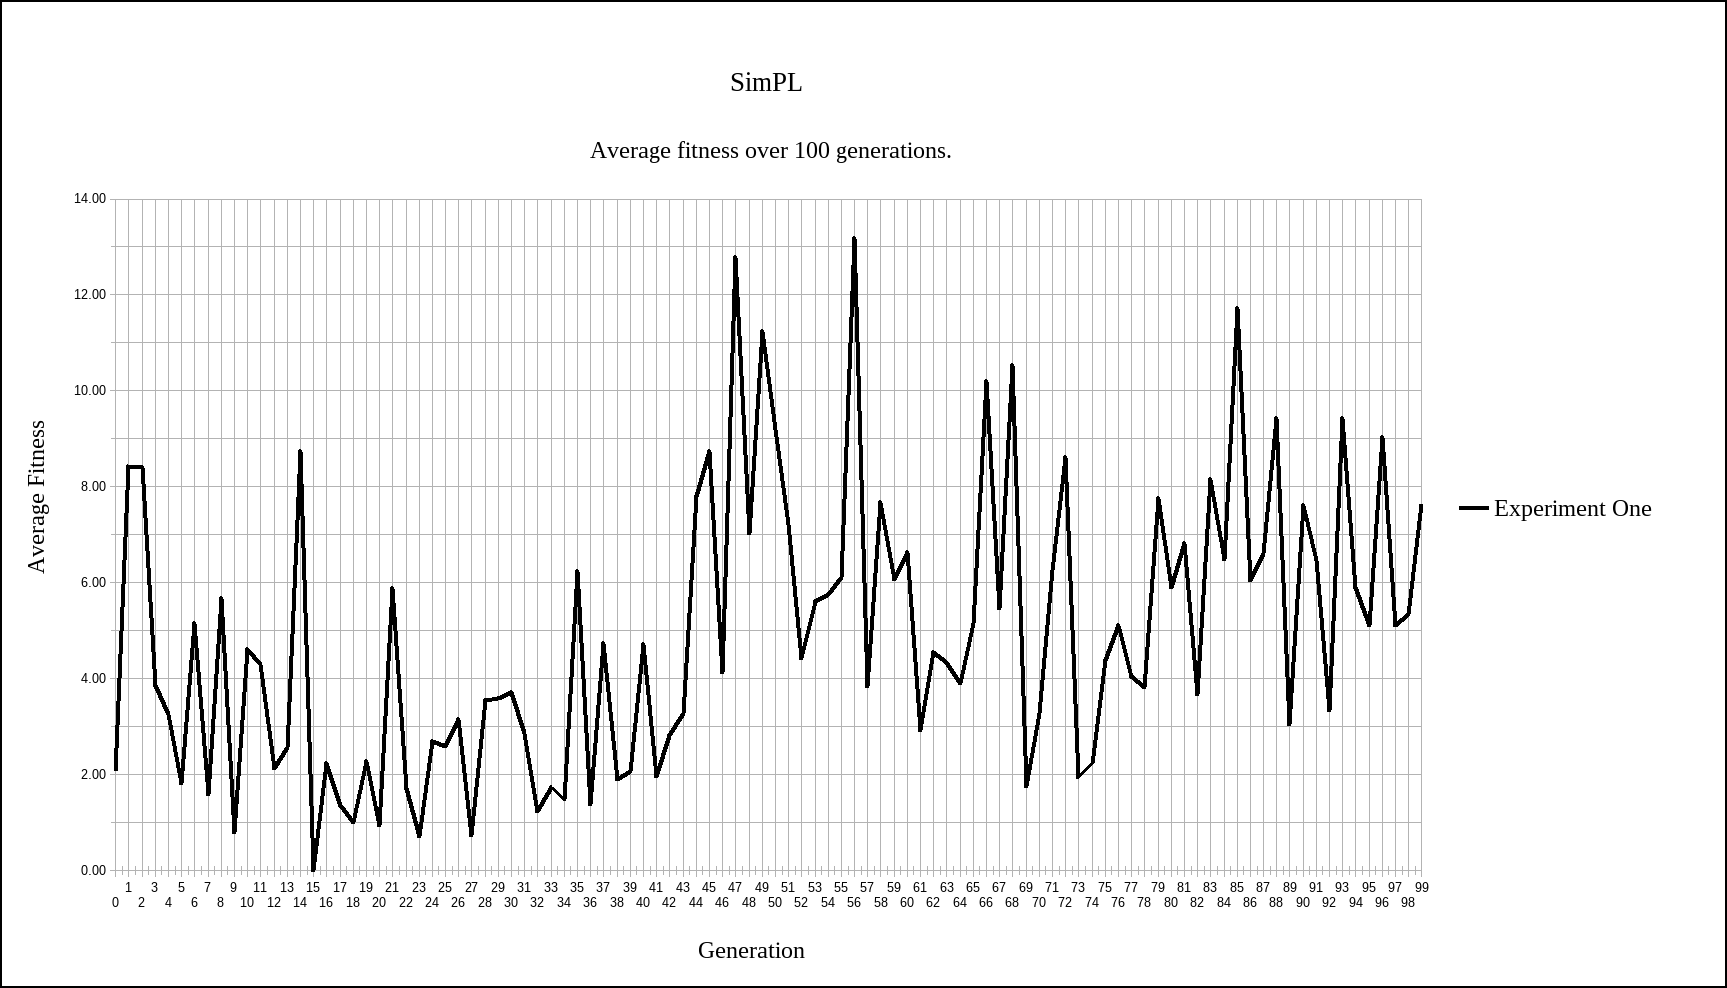
\includegraphics[width=1\textwidth]{figures/exp1_avg_fit.png}
  \caption{Here you see the average fitness over 100 generations for experiment one.}
  \label{fig:exp1_avg_fit}
\end{figure}

\begin{figure}[H]  
  \centering
  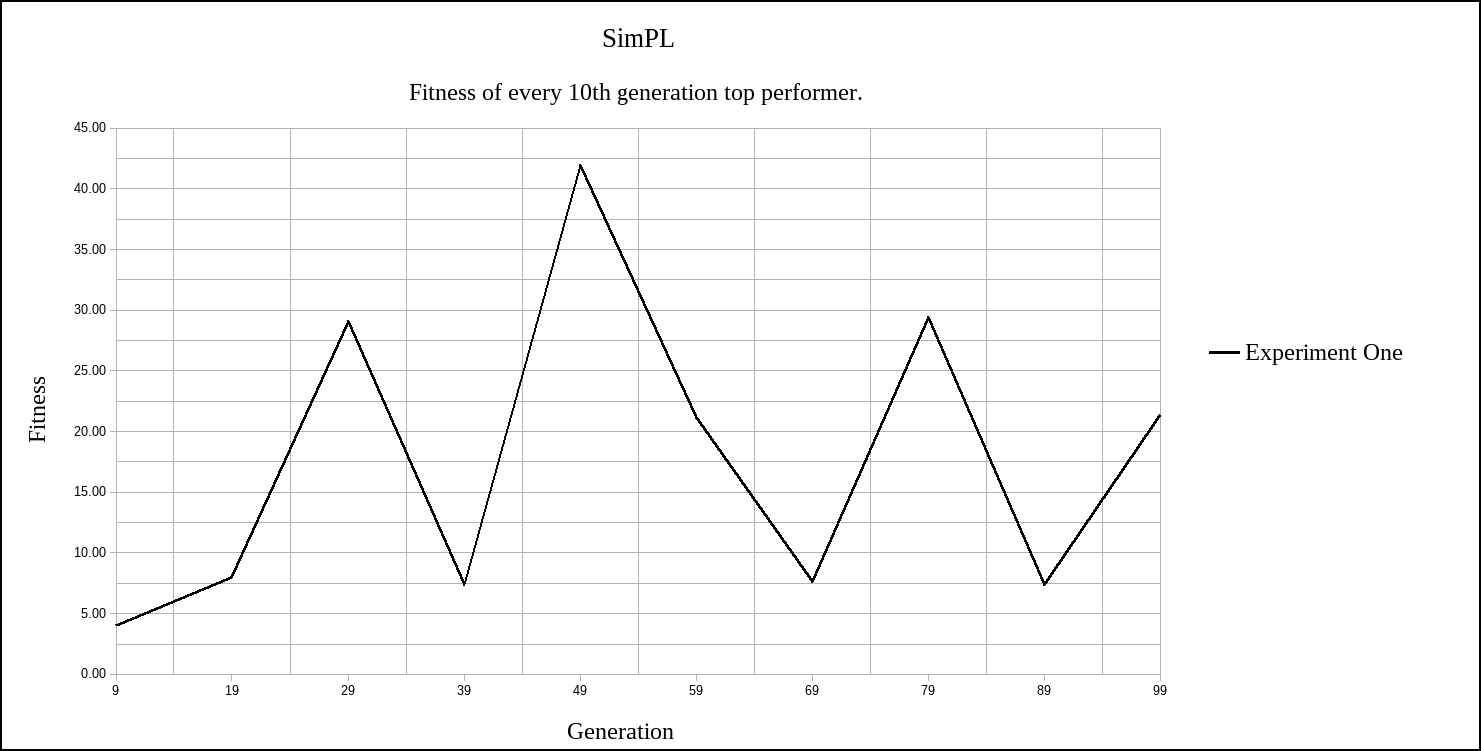
\includegraphics[width=1\textwidth]{figures/exp1_10_tops.png}
  \caption{Here you see the fitness of every 10th generation top performer for experiment one.}
  \label{fig:exp1_10_tops}
\end{figure}

\begin{figure}[H]  
  \centering
  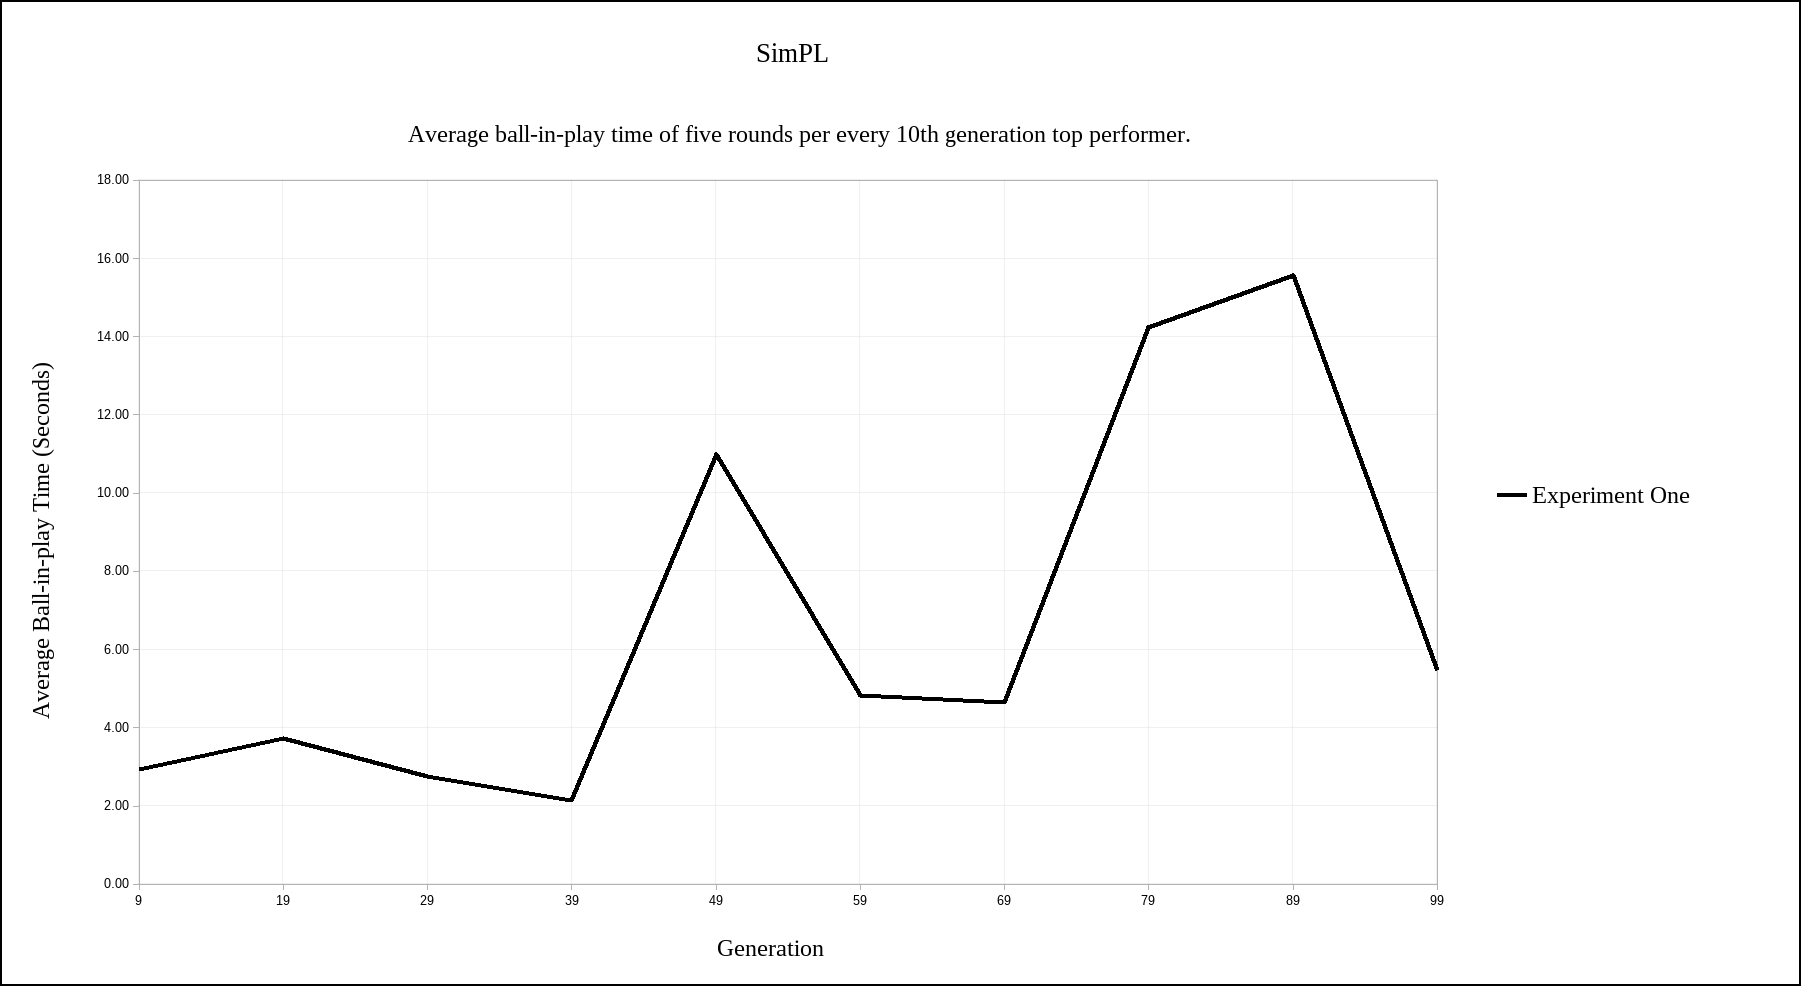
\includegraphics[width=1\textwidth]{figures/exp1_10_tops_times.png}
  \caption{Here you see the average ball-in-play time (in seconds) of five rounds per every 10th generation top performer for experiment one.}
  \label{fig:exp1_10_tops_times}
\end{figure}

\subsection{Experiment two: use of a simplified fitness function, use of rank fitness in selection, higher crossover probability, mutation probability based on the number of genes per genome, and a Gaussian distribution sample mutation step.}

Experiment two (Figures \ref{fig:exp2_avg_fit}-\ref{fig:exp2_10_tops_times}) shows marked improvement in average fitness to generation 20, and then a more gradual improvement for the remaining 80 generations. The average ball-in-play times improve dramatically from 10.1 seconds to 37.8 seconds within the first 20 generations, but levels off and does not show marked improvement for the remainder of the experiment.

\begin{figure}[H]  
  \centering
  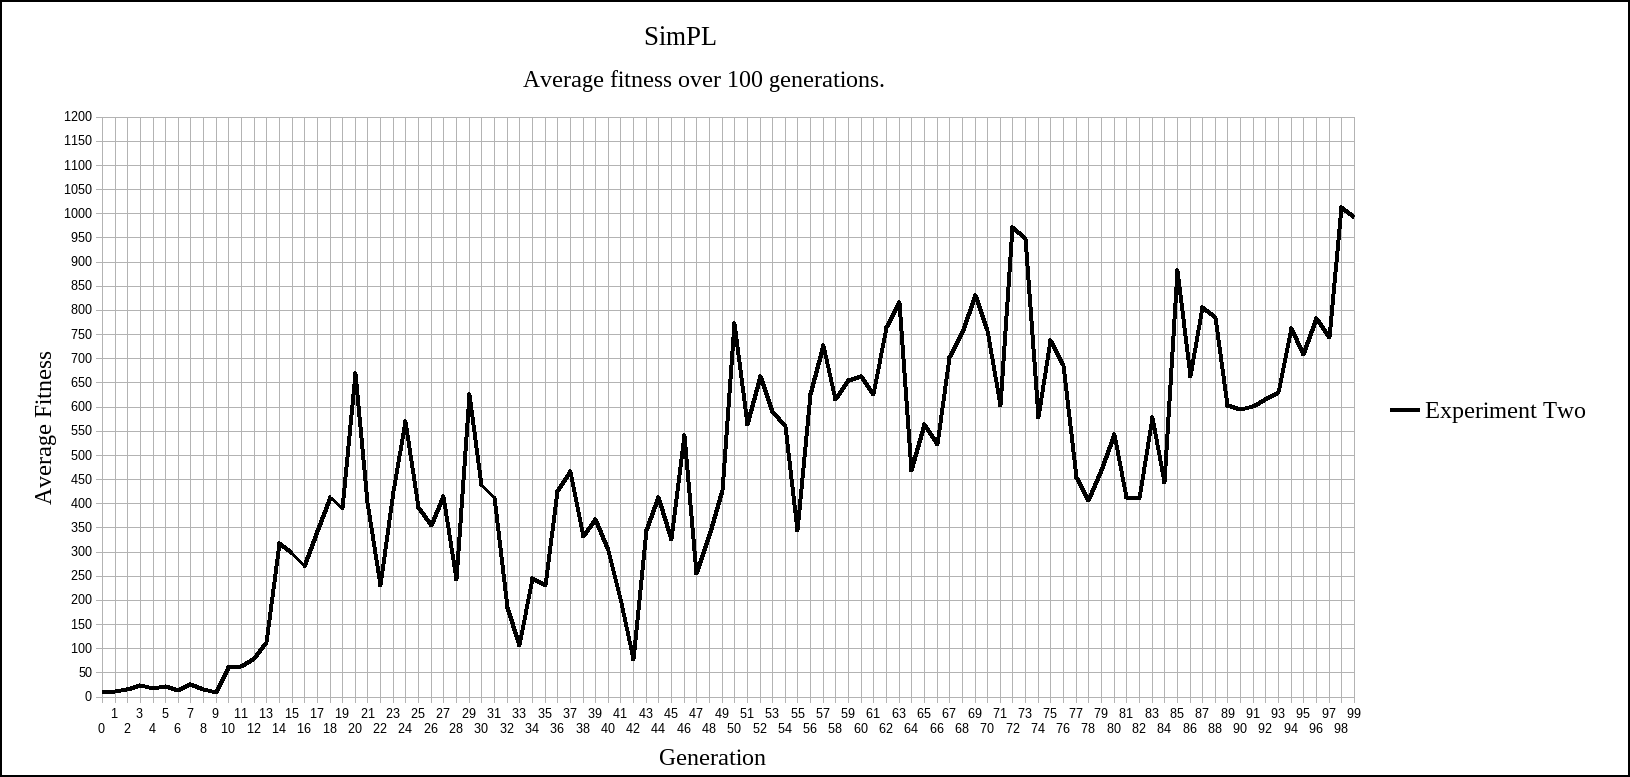
\includegraphics[width=1\textwidth]{figures/exp2_avg_fit.png}
  \caption{Here you see the average fitness over 100 generations for experiment two.}
  \label{fig:exp2_avg_fit}
\end{figure}

\begin{figure}[H]  
  \centering
  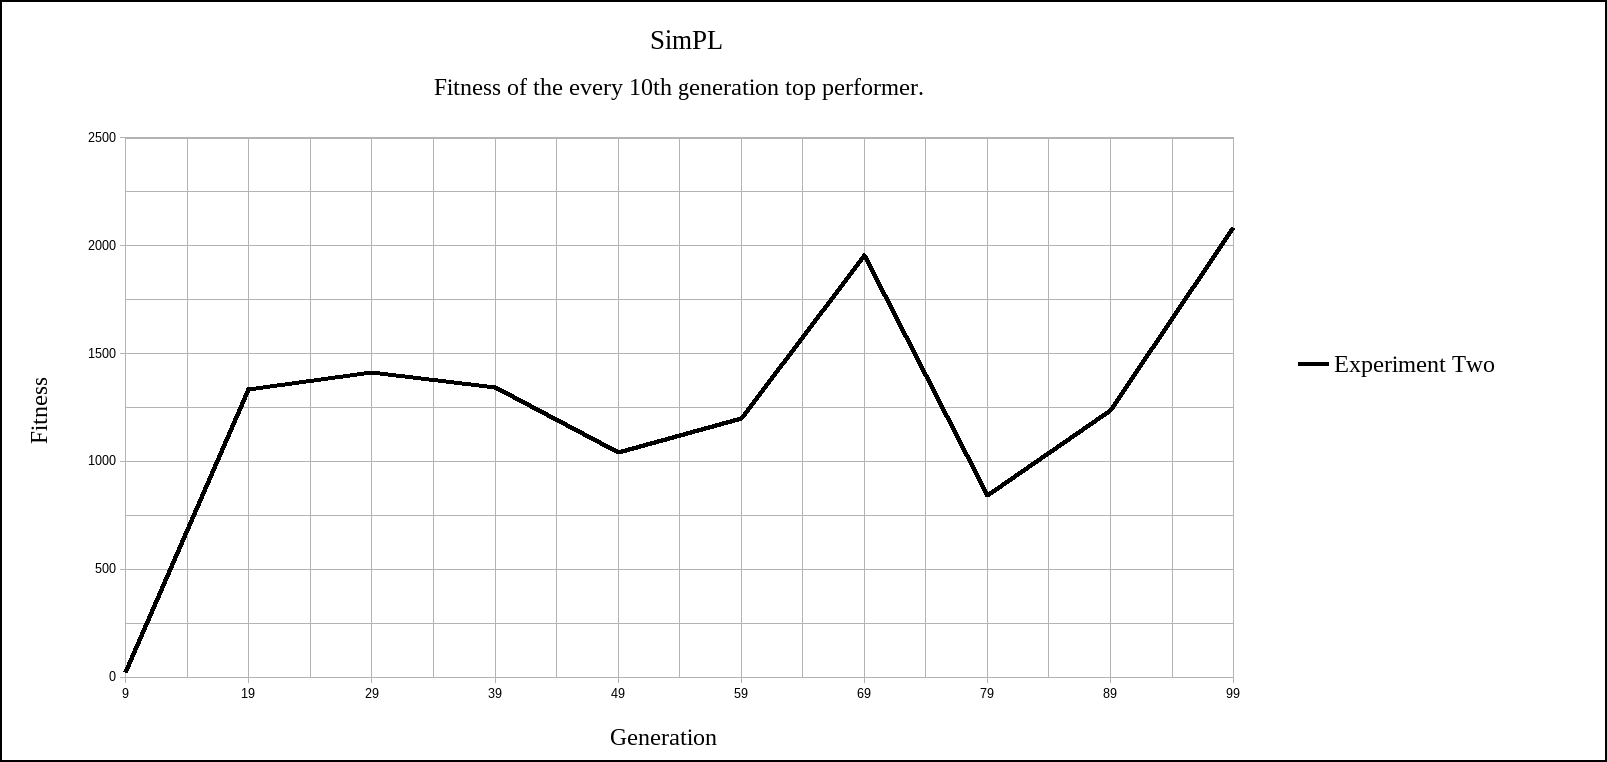
\includegraphics[width=1\textwidth]{figures/exp2_10_tops.png}
  \caption{Here you see the fitness of every 10th generation top performer for experiment two.}
  \label{fig:exp2_10_tops}
\end{figure}

\begin{figure}[H]  
  \centering
  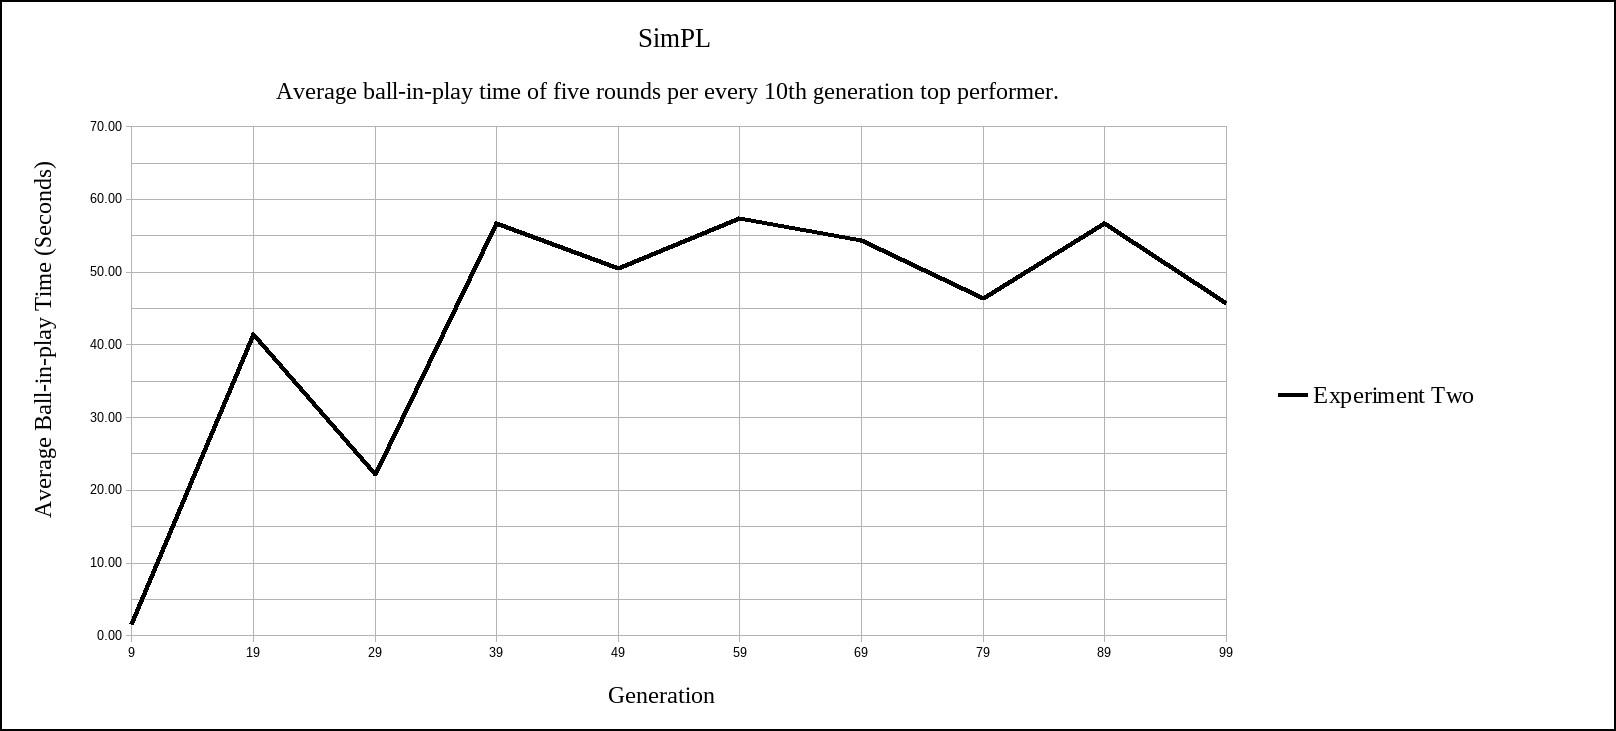
\includegraphics[width=1\textwidth]{figures/exp2_10_tops_times.png}
  \caption{Here you see the average ball-in-play time (in seconds) of five rounds per every 10th generation top performer for experiment two.}
  \label{fig:exp2_10_tops_times}
\end{figure}

\subsection{Experiment three: self-adaptation of crossover and mutation probabilities with the crossover and mutation operators working in parallel.}

Experiment three (Figures \ref{fig:exp3_avg_fit}-\ref{fig:exp3_10_tops_times}) shows initial improvement in average fitness for the first 12 generations, but then oscillates and does not show measurable improvement for the rest of the experiment. This result is reflected in the average ball-in-play time metric, which starts at 35.7314 seconds and oscillates but does not trend significantly. Figure \ref{fig:exp3_self_adapt} illustrates the self-adaptation of the crossover and mutation probabilities, as chosen by the algorithm at run-time. Although the proportions change, they do not appear to correlate with the fitness or average ball-in-play time results.

\begin{figure}[H]  
  \centering
  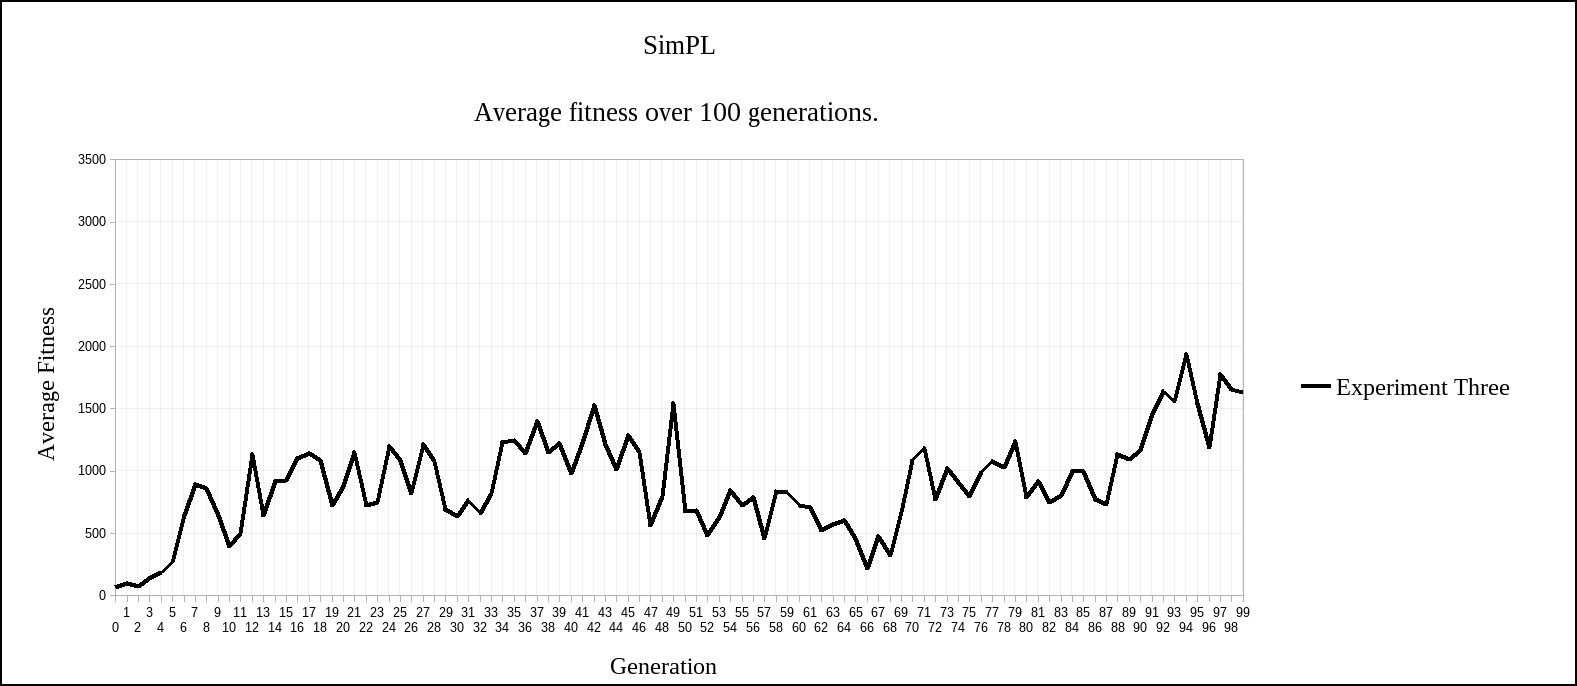
\includegraphics[width=1\textwidth]{figures/exp3_avg_fit.png}
  \caption{Here you see the average fitness over 100 generations for experiment three.}
  \label{fig:exp3_avg_fit}
\end{figure}

The crossover and mutation probabilities were both initially set to $0.5$ before the start of the experiment. After the experiment was over, the genetic algorithm self-adapted the crossover probability to $0.7816$ and self-adapted the mutation probability to $0.2184$. You'll notice in Figure \ref{fig:exp3_self_adapt} that the mutation probability overtook the crossover probability at first but the two probabilities eventually diverged with mutation becoming less probable and crossover becoming more probable as the genetic algorithm produced fitter generations. This outcome is almost the exact opposite of the outcome shown in \cite{self_adapt}.

\begin{figure}[H]  
  \centering
  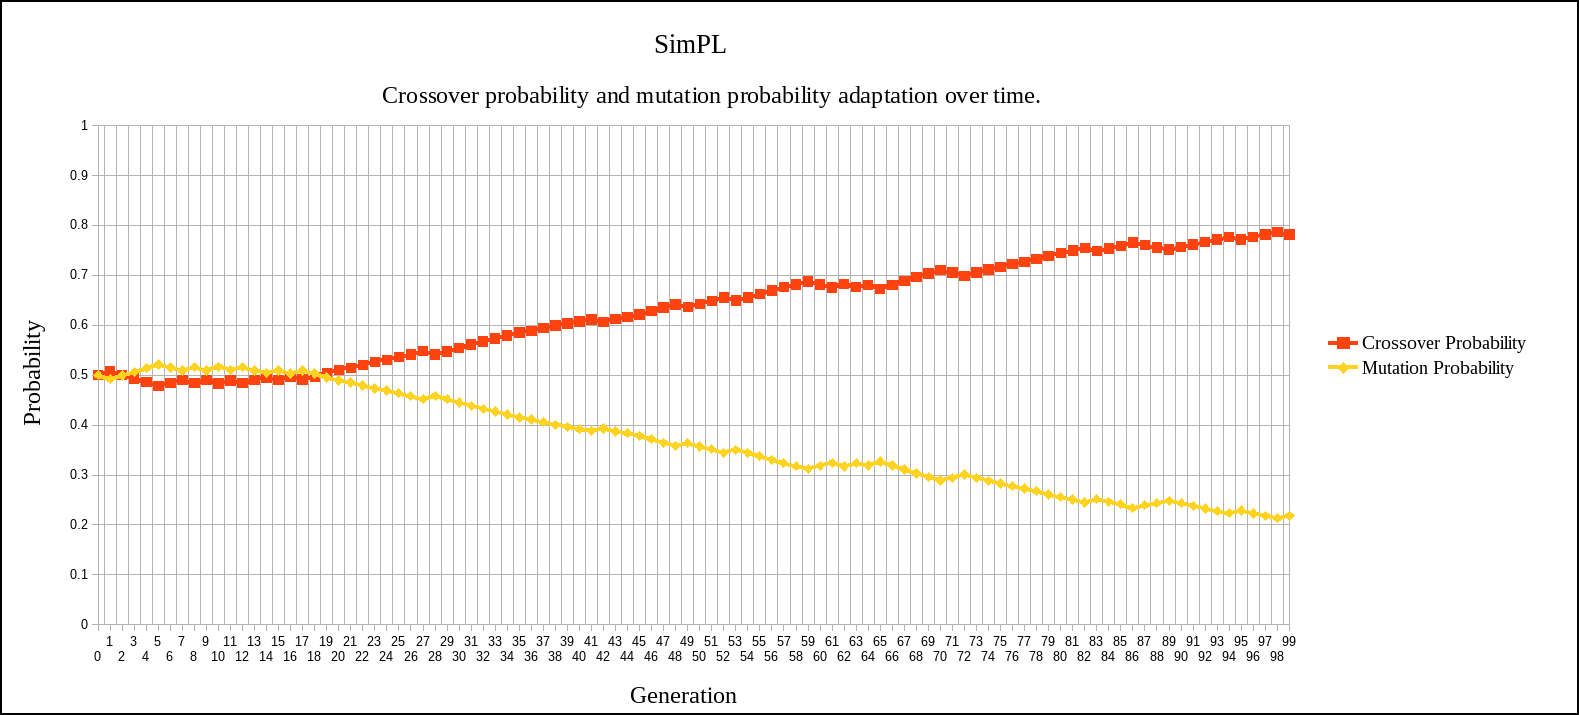
\includegraphics[width=1\textwidth]{figures/exp3_self_adapt.png}
  \caption{Here you see the self-adaptation of the crossover and mutation probabilities for experiment three.}
  \label{fig:exp3_self_adapt}
\end{figure}

\begin{figure}[H]  
  \centering
  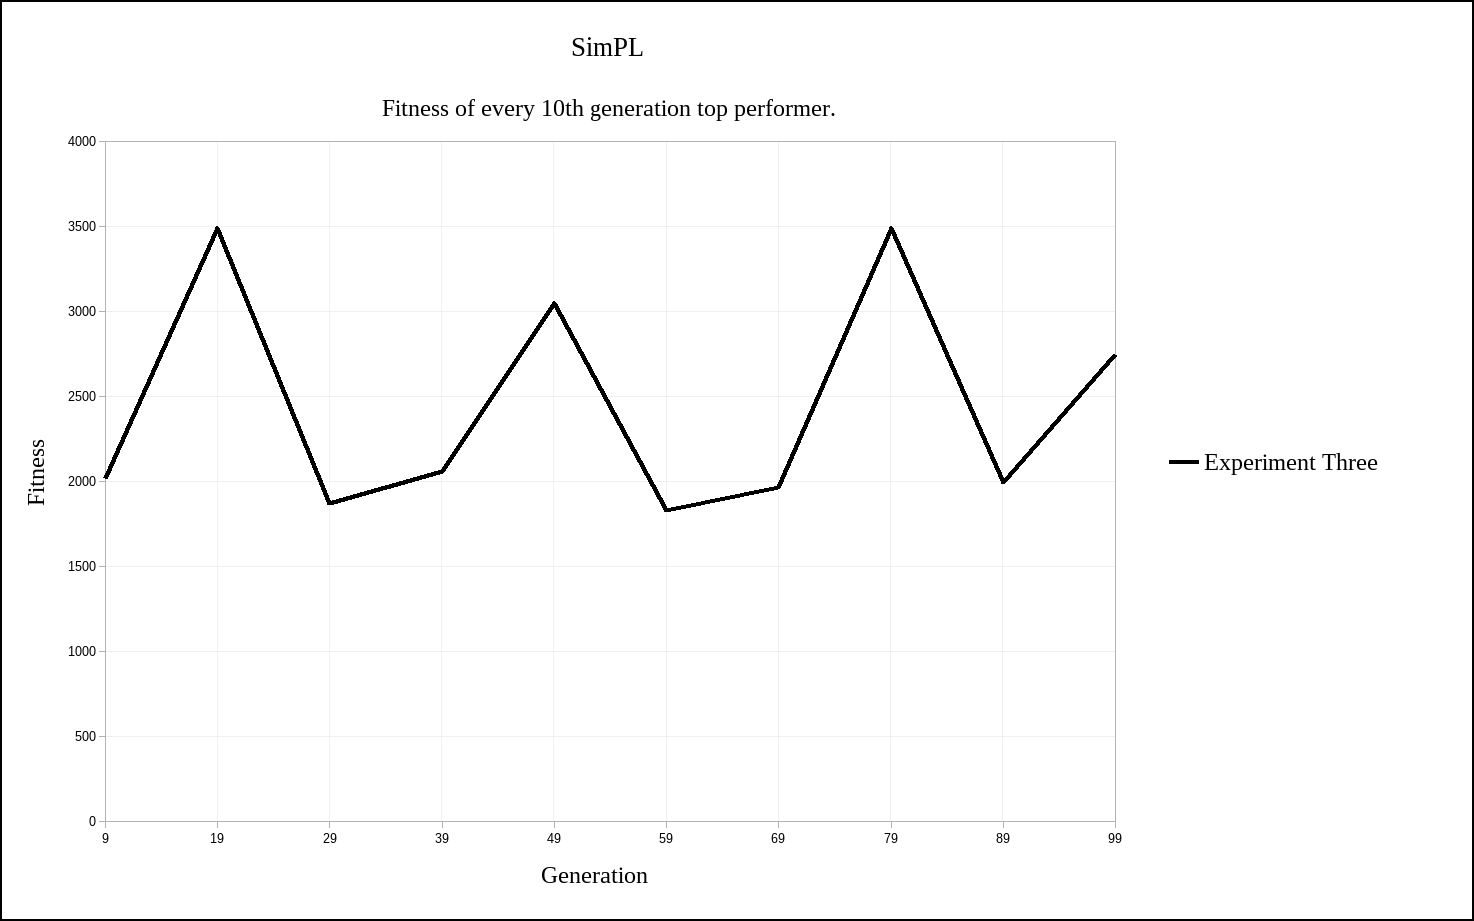
\includegraphics[width=1\textwidth]{figures/exp3_10_tops.png}
  \caption{Here you see the fitness of every 10th generation top performer for experiment three.}
  \label{fig:exp3_10_tops}
\end{figure}

\begin{figure}[H]  
  \centering
  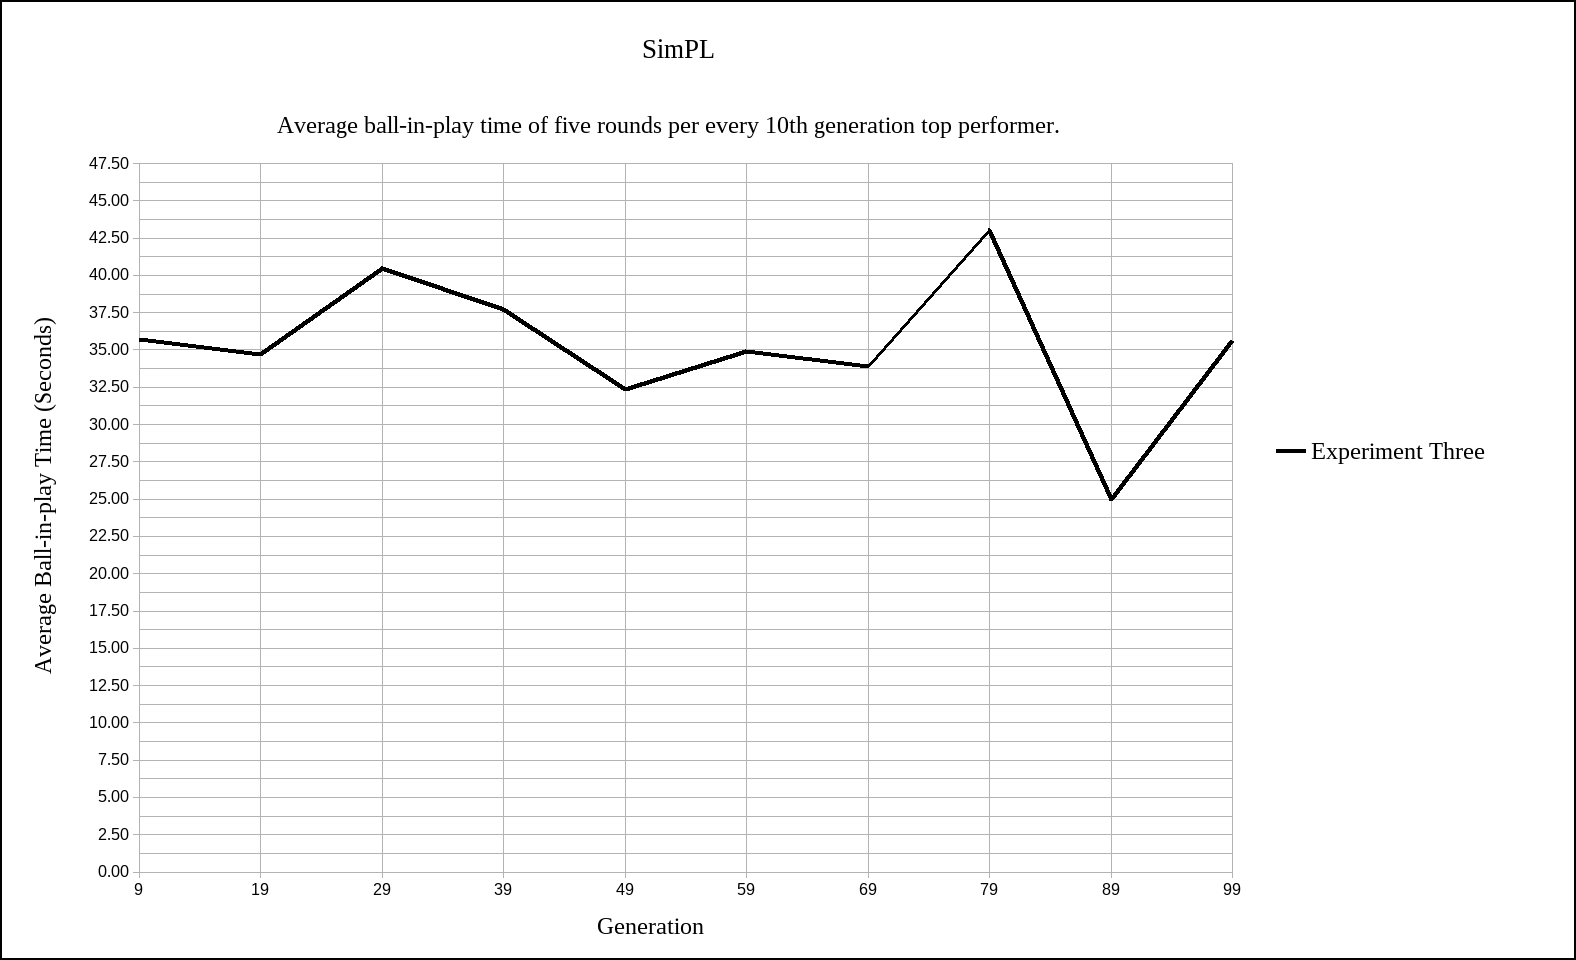
\includegraphics[width=1\textwidth]{figures/exp3_10_tops_times.png}
  \caption{Here you see the average ball-in-play time (in seconds) of five rounds per every 10th generation top performer for experiment three.}
  \label{fig:exp3_10_tops_times}
\end{figure}

\subsection{Experiment four: static crossover and mutation probabilities with the crossover and mutation operators working in parallel.}

Experiment four (Figures \ref{fig:exp4_avg_fit}-\ref{fig:exp4_10_tops_times}) produces similar results, with initial improvement in average fitness for the first 10 generations, but oscillation thereafter. However, the mean of the average ball-in-play times was 37.28646 seconds, over the mean 35.33994 seconds shown for the player learned in Experiment three and the mean 34.18604 seconds in Experiment two.

\begin{figure}[H]  
  \centering
  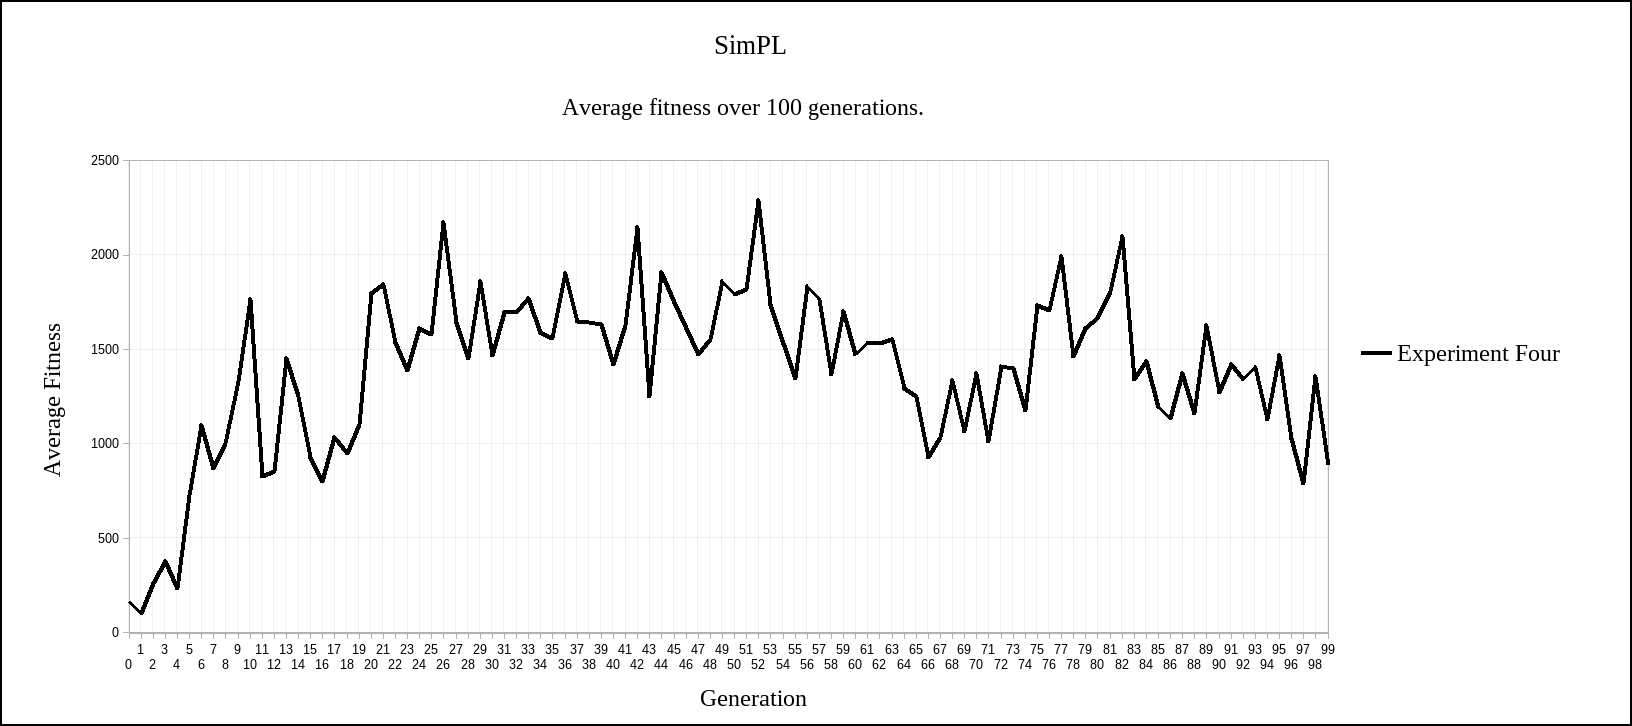
\includegraphics[width=1\textwidth]{figures/exp4_avg_fit.png}
  \caption{Here you see the average fitness over 100 generations for experiment four.}
  \label{fig:exp4_avg_fit}
\end{figure}

\begin{figure}[H]  
  \centering
  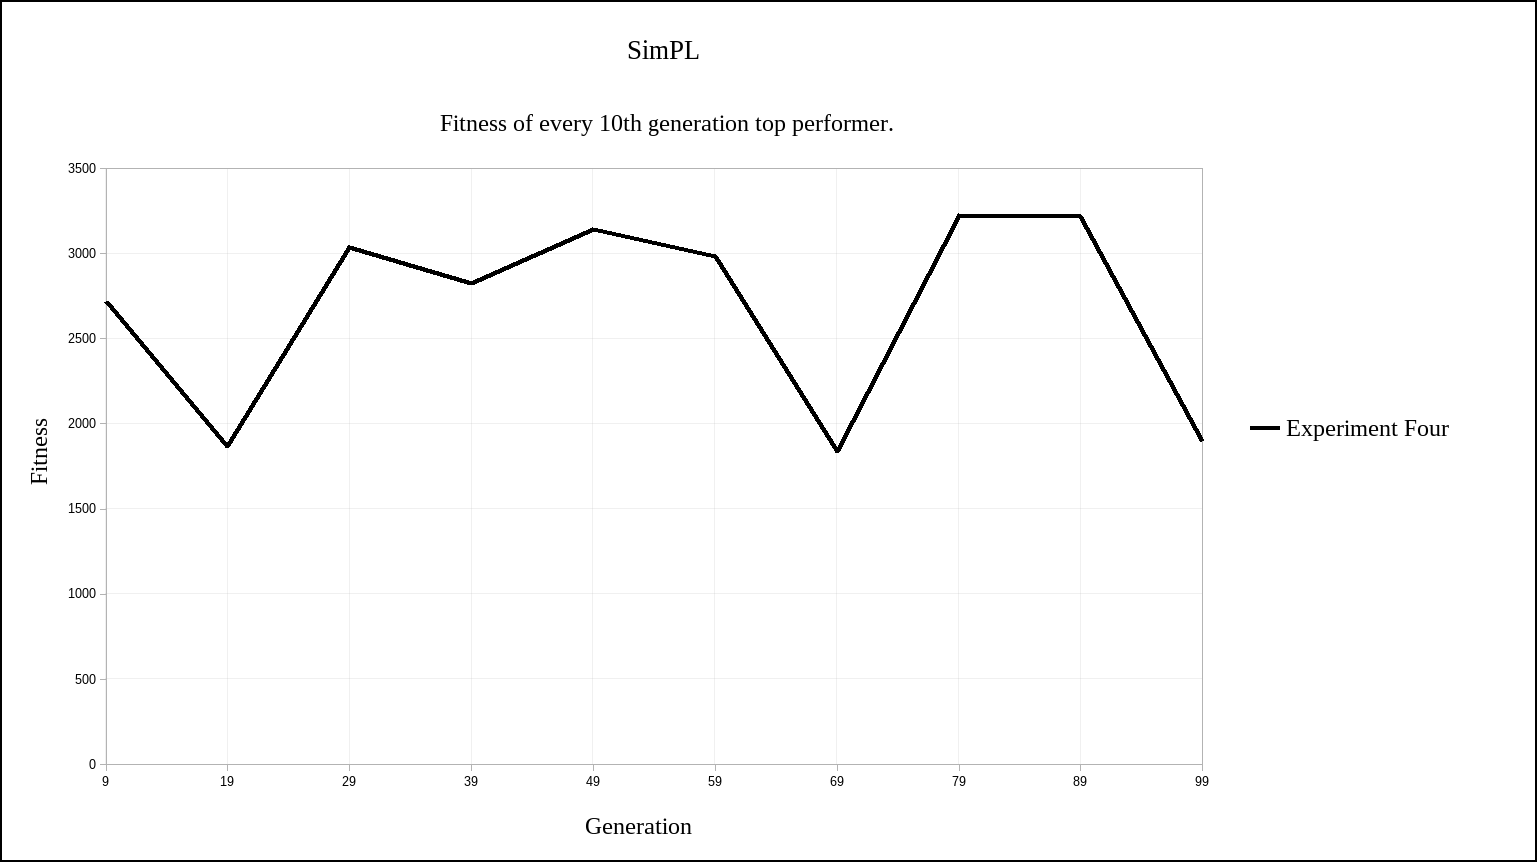
\includegraphics[width=1\textwidth]{figures/exp4_10_tops.png}
  \caption{Here you see the fitness of every 10th generation top performer for experiment four.}
  \label{fig:exp4_10_tops}
\end{figure}

\begin{figure}[H]  
  \centering
  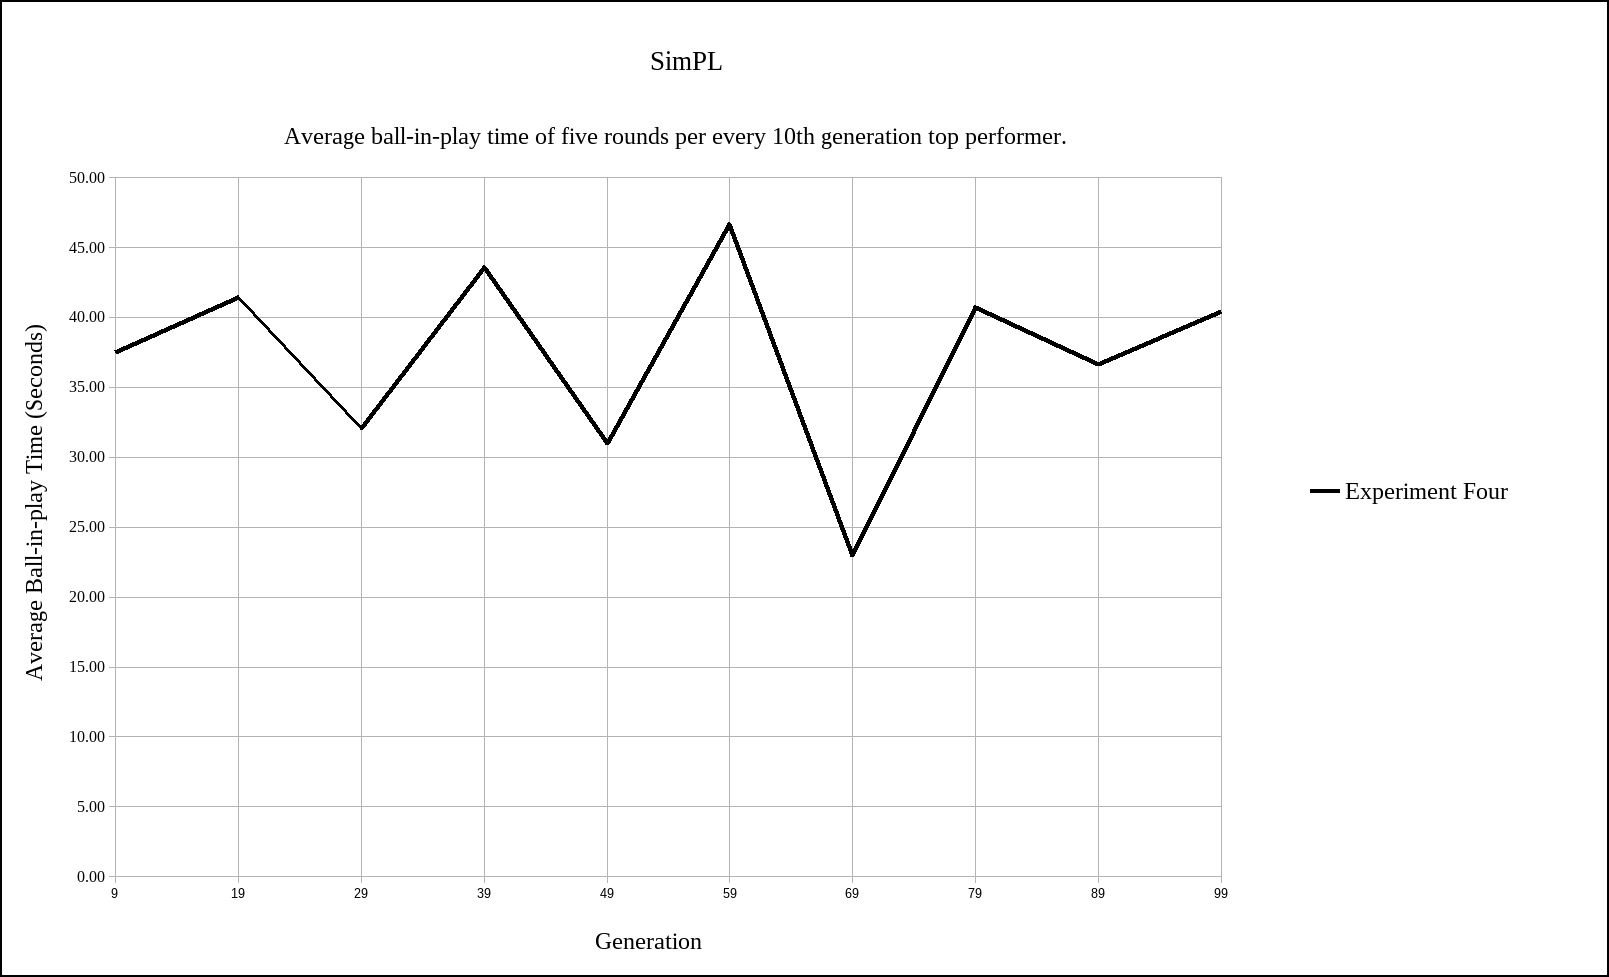
\includegraphics[width=1\textwidth]{figures/exp4_10_tops_times.png}
  \caption{Here you see the average ball-in-play time (in seconds) of five rounds per every 10th generation top performer for experiment four.}
  \label{fig:exp4_10_tops_times}
\end{figure}

\subsection{Experiment five: static crossover and mutation probabilities with the crossover and mutation operators working in sequence.}

Experiment five (Figures \ref{fig:exp5_avg_fit}-\ref{fig:exp5_10_tops_times}) shows more gradual improvement in average fitness over the first 31 generations. Overall, the mean of the average ball-in-play times was 37.91126 seconds---higher than that of Experiment four.

\begin{figure}[H]  
  \centering
  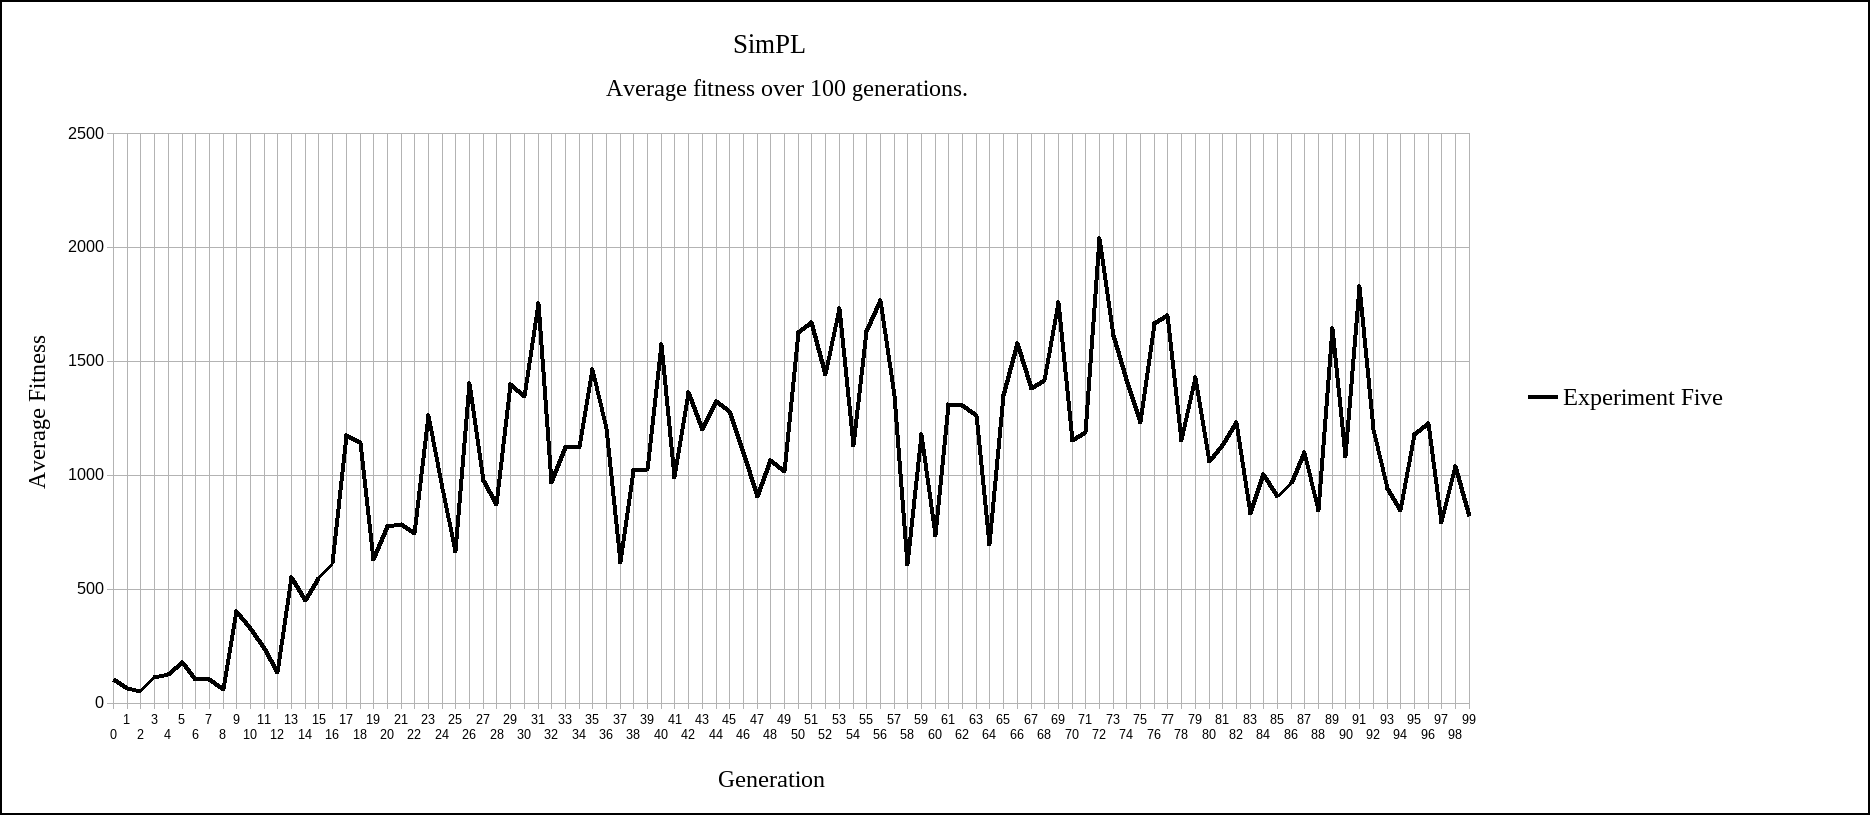
\includegraphics[width=1\textwidth]{figures/exp5_avg_fit.png}
  \caption{Here you see the average fitness over 100 generations for experiment five.}
  \label{fig:exp5_avg_fit}
\end{figure}

\begin{figure}[H]  
  \centering
  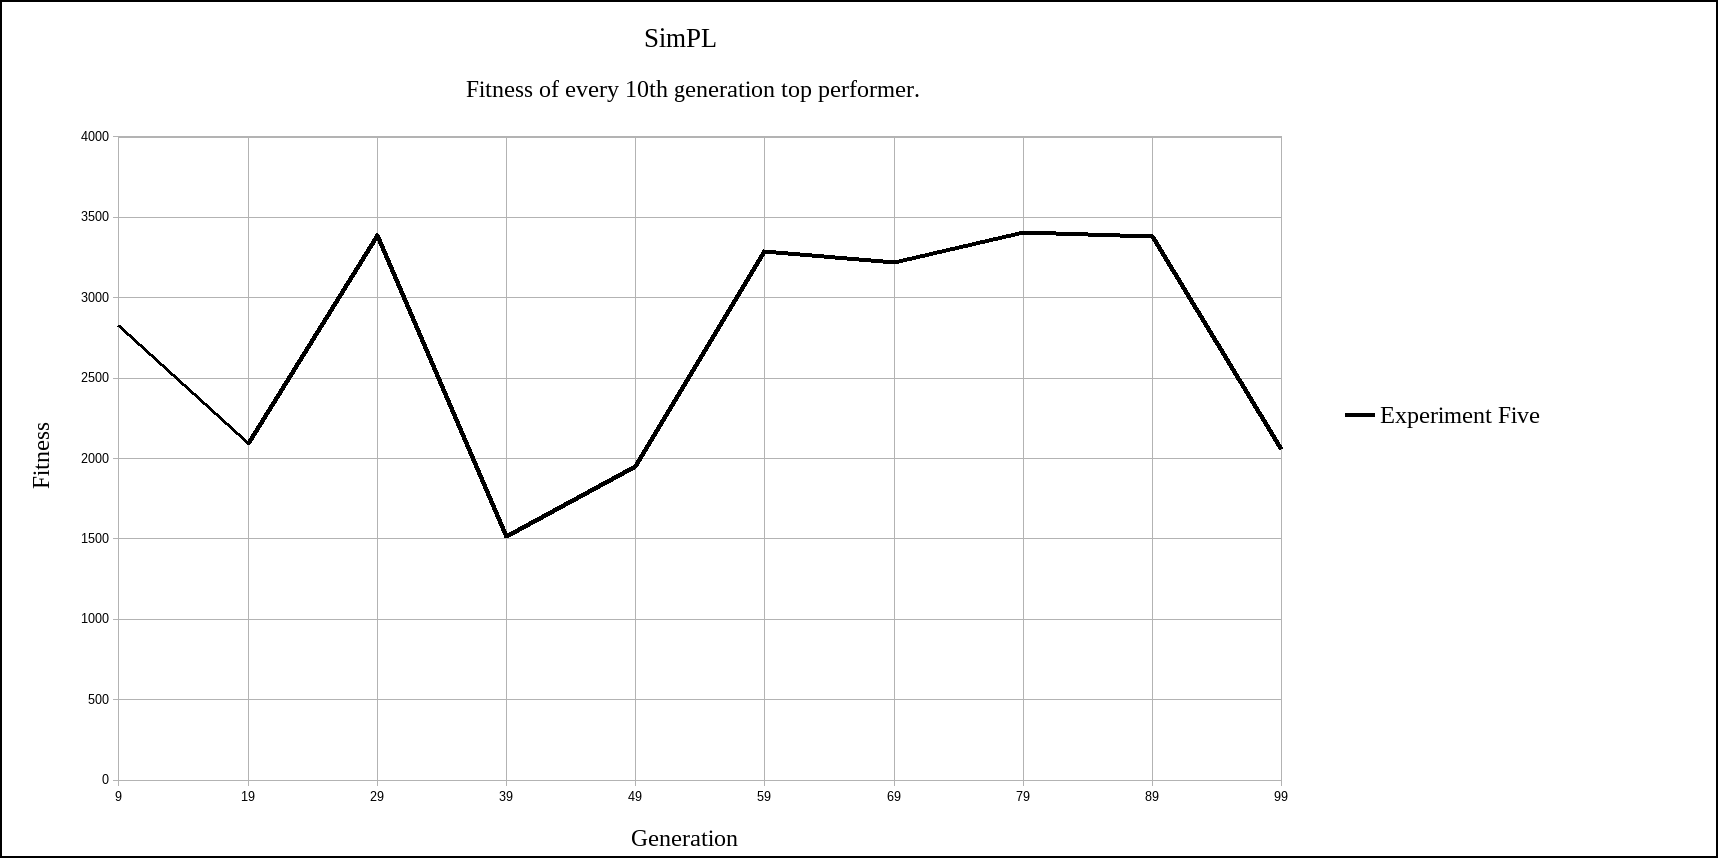
\includegraphics[width=1\textwidth]{figures/exp5_10_tops.png}
  \caption{Here you see the fitness of every 10th generation top performer for experiment five.}
  \label{fig:exp5_10_tops}
\end{figure}

\begin{figure}[H]  
  \centering
  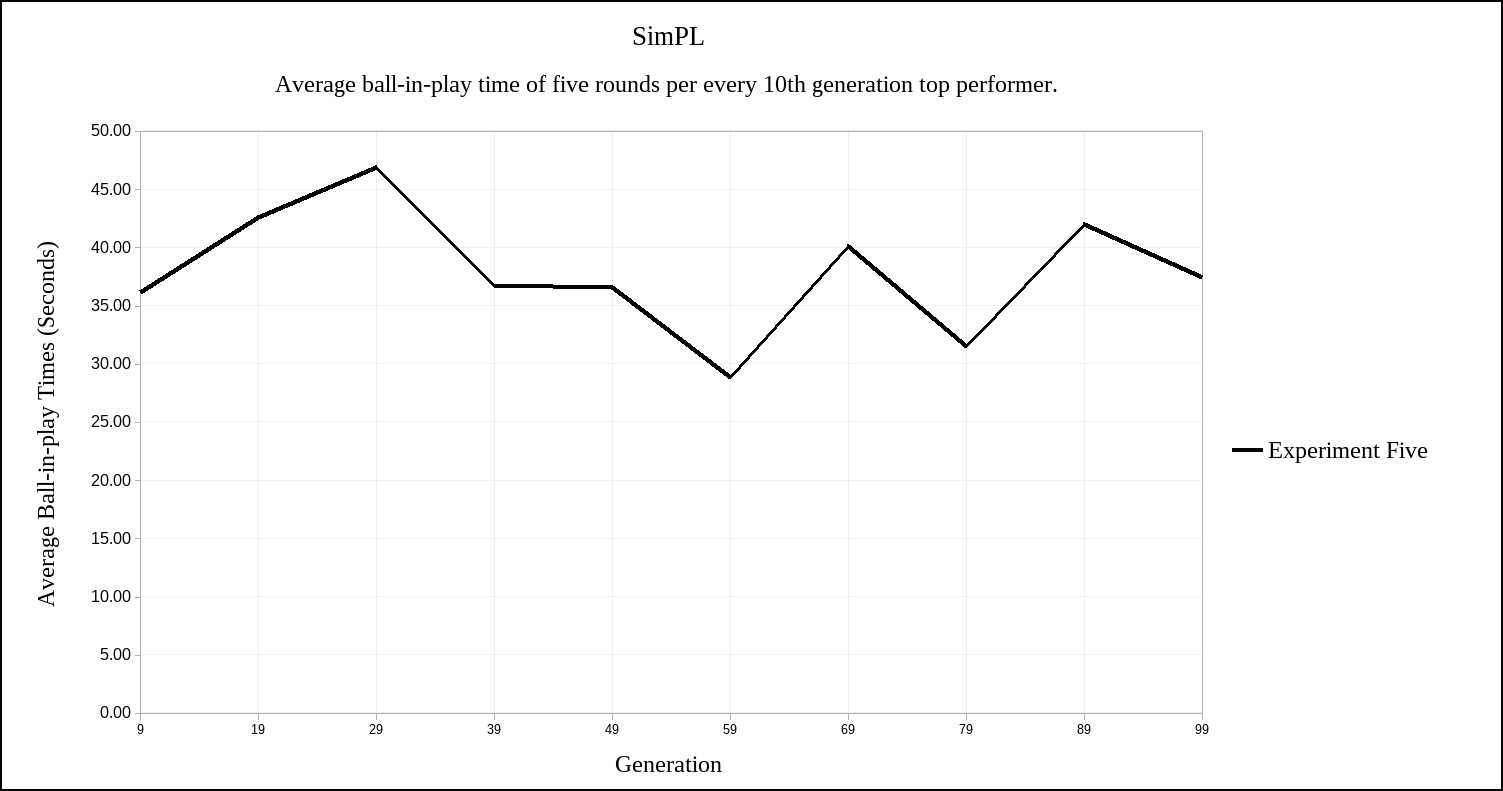
\includegraphics[width=1\textwidth]{figures/exp5_10_tops_times.png}
  \caption{Here you see the average ball-in-play time (in seconds) of five rounds per every 10th generation top performer for experiment five.}
  \label{fig:exp5_10_tops_times}
\end{figure}

\subsection{Experiment six: fitness and ball-in-play upper bound.}

Experiment six (Figures \ref{fig:exp6_avg_fit}-\ref{fig:exp6_10_tops_times}) illustrates the \textit{perfect} results possible of a player who always behaves correctly. These metrics demonstrate optimal values, which can be considered targets for the evolution experiments. The mean of the average ball-in-play times was 40.01528 seconds, which means that Experiment five (above) comes closest to optimal performance.

\begin{figure}[H]  
  \centering
  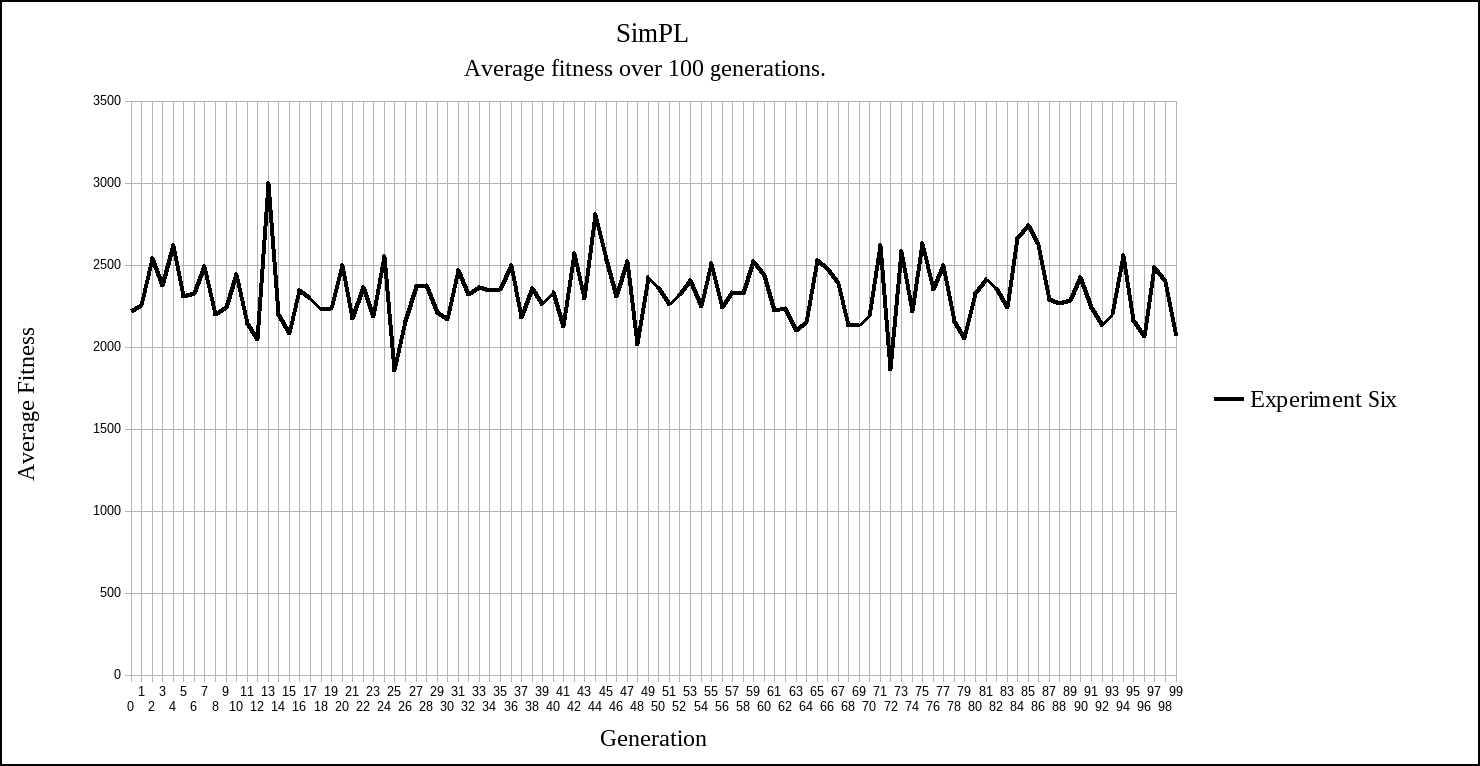
\includegraphics[width=1\textwidth]{figures/exp6_avg_fit.png}
  \caption{Here you see the average fitness over 100 generations for experiment six.}
  \label{fig:exp6_avg_fit}
\end{figure}

\begin{figure}[H]  
  \centering
  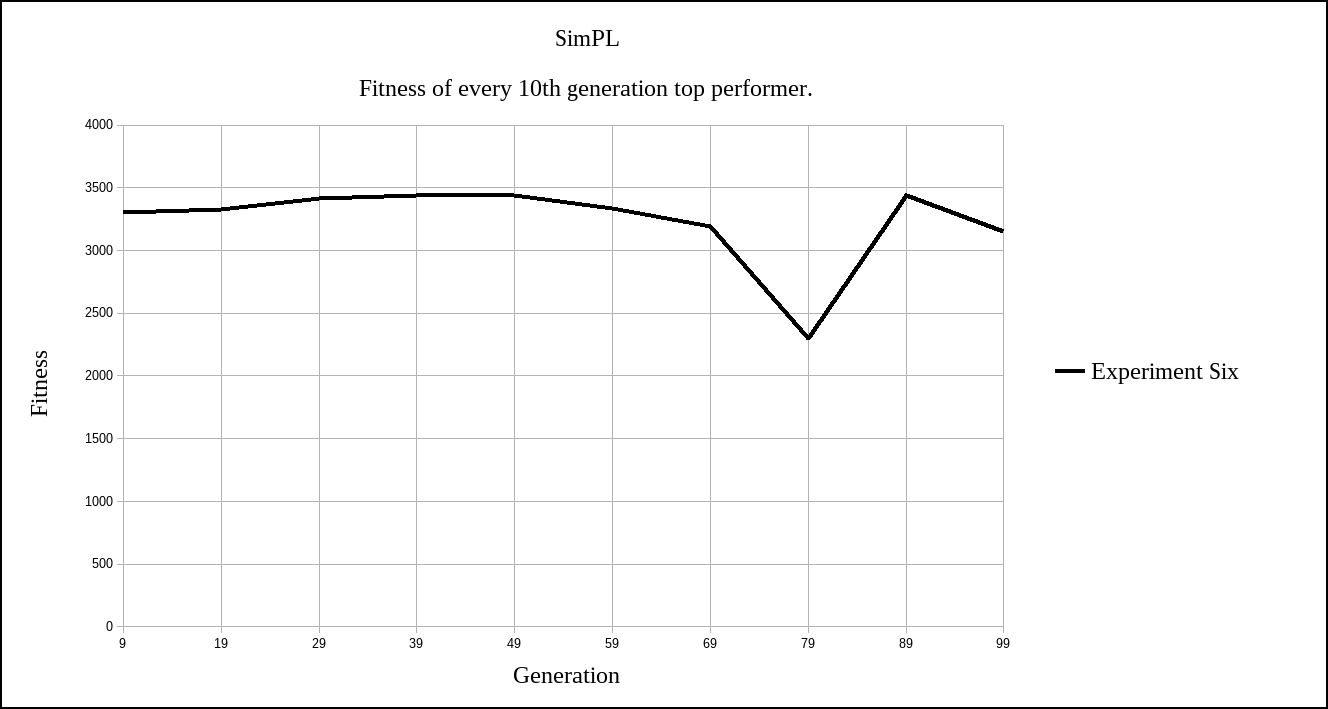
\includegraphics[width=1\textwidth]{figures/exp6_10_tops.png}
  \caption{Here you see the fitness of every 10th generation top performer for experiment six.}
  \label{fig:exp6_10_tops}
\end{figure}

\begin{figure}[H]  
  \centering
  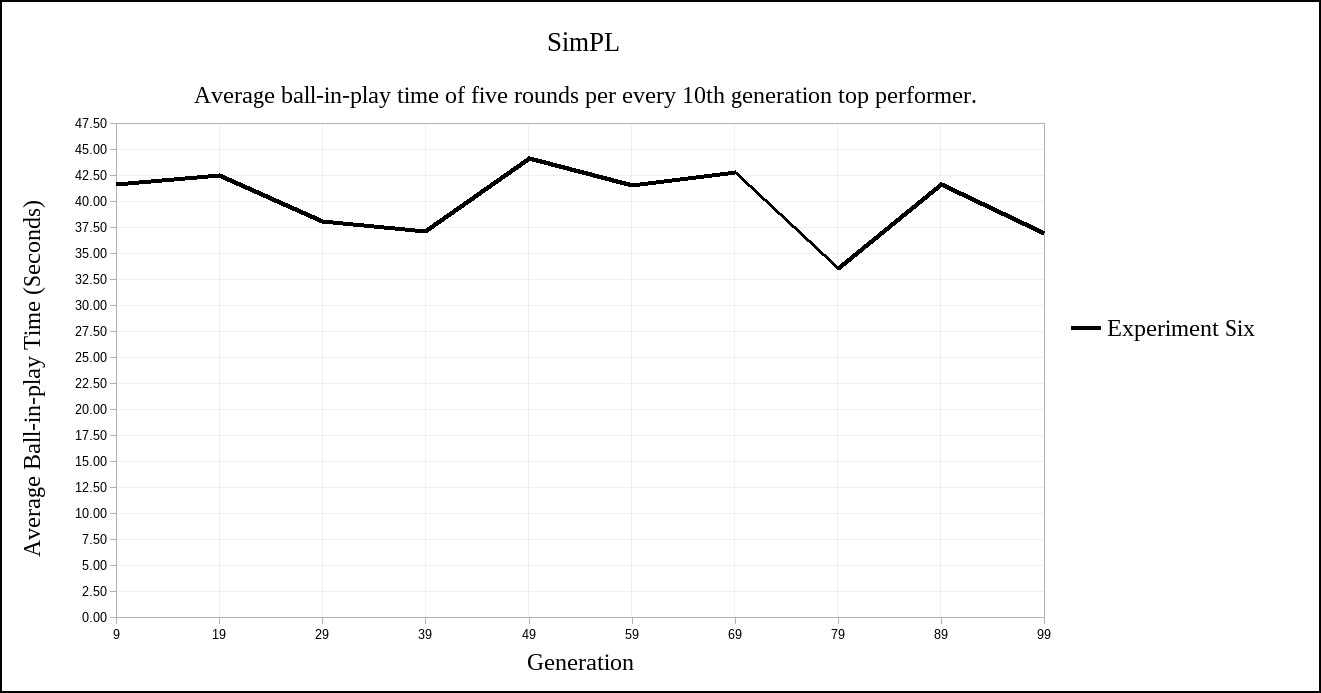
\includegraphics[width=1\textwidth]{figures/exp6_10_tops_times.png}
  \caption{Here you see the average ball-in-play time (in seconds) of five rounds per every 10th generation top performer for experiment six.}
  \label{fig:exp6_10_tops_times}
\end{figure}

\subsection{Experiment seven: random paddles.}

Experiment seven (Figures \ref{fig:exp7_avg_fit}-\ref{fig:exp7_10_tops_times}) illustrates the results of a player who behaves randomly. This provides an example of worst case metrics. The mean of the average average ball-in-play times was 5.2656 seconds, which is comparable to the first-generation games of the evolved players.

\begin{figure}[H]  
  \centering
  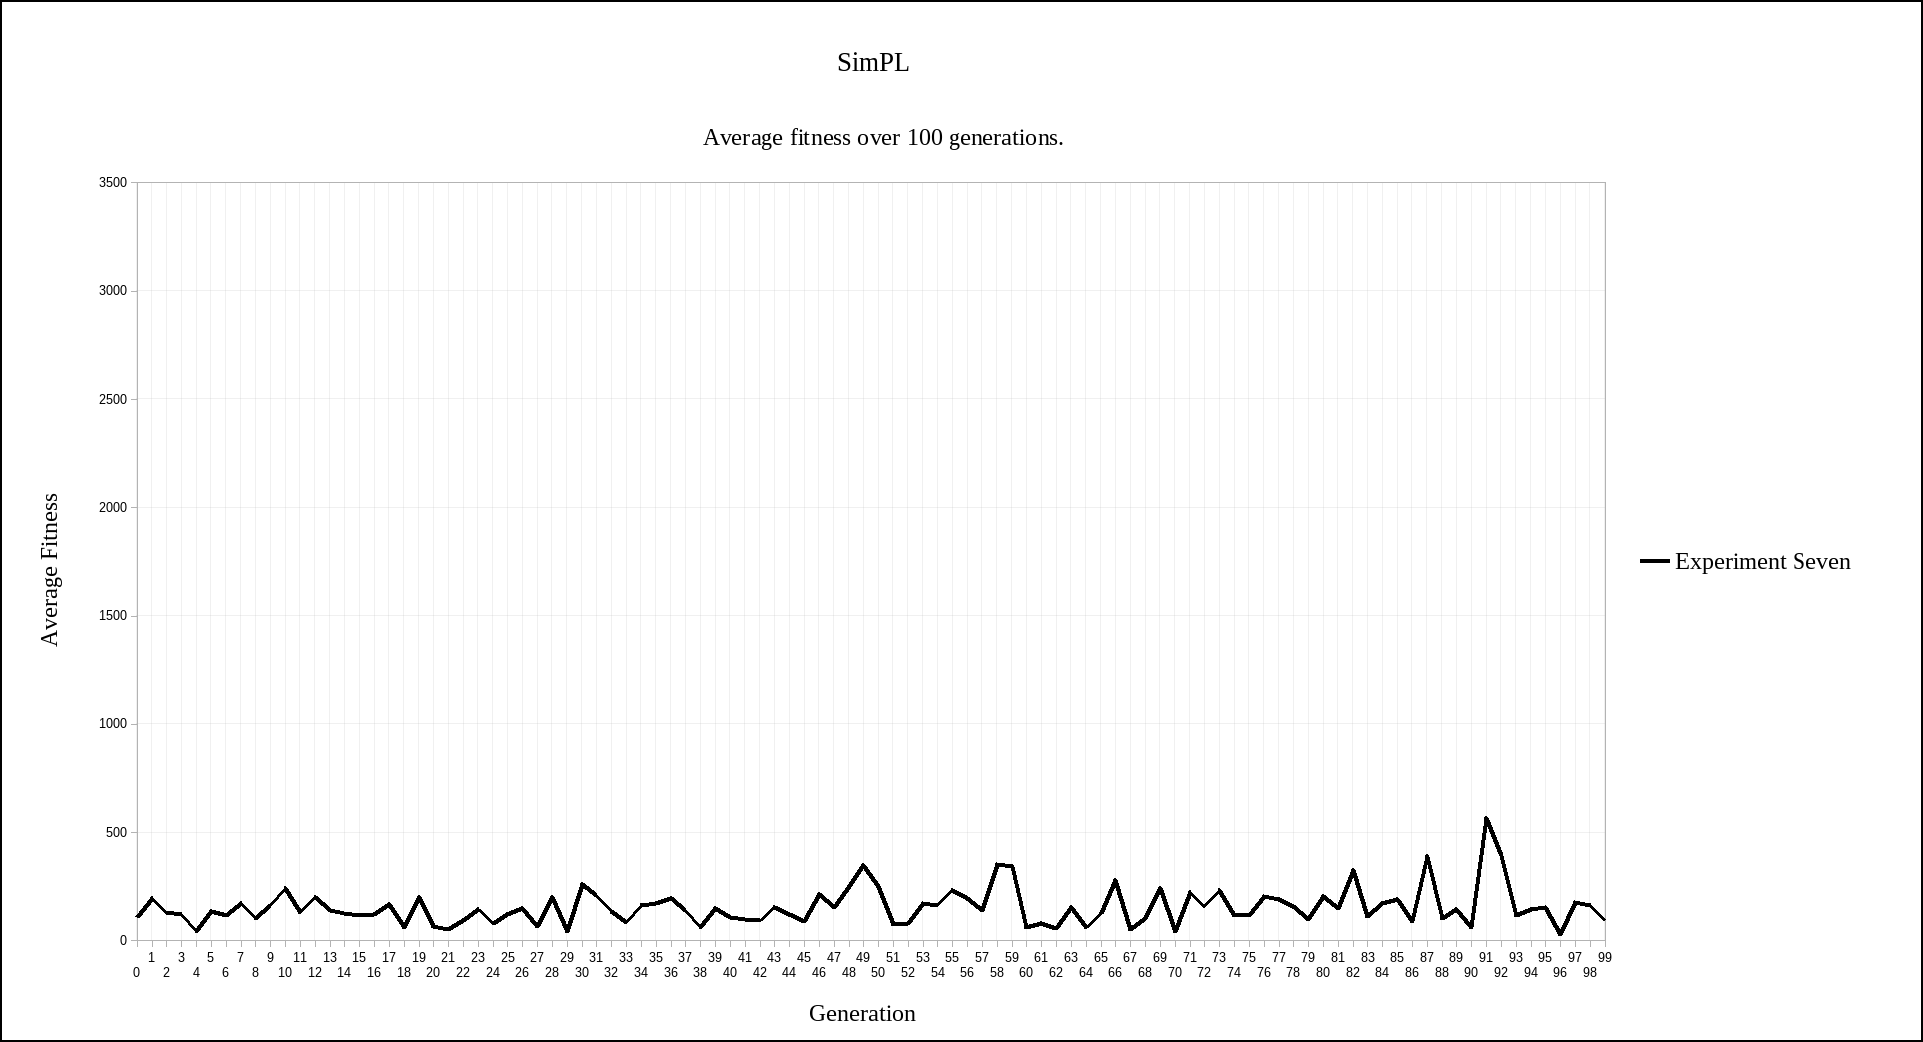
\includegraphics[width=1\textwidth]{figures/exp7_avg_fit.png}
  \caption{Here you see the average fitness over 100 generations for experiment seven.}
  \label{fig:exp7_avg_fit}
\end{figure}

\begin{figure}[H]  
  \centering
  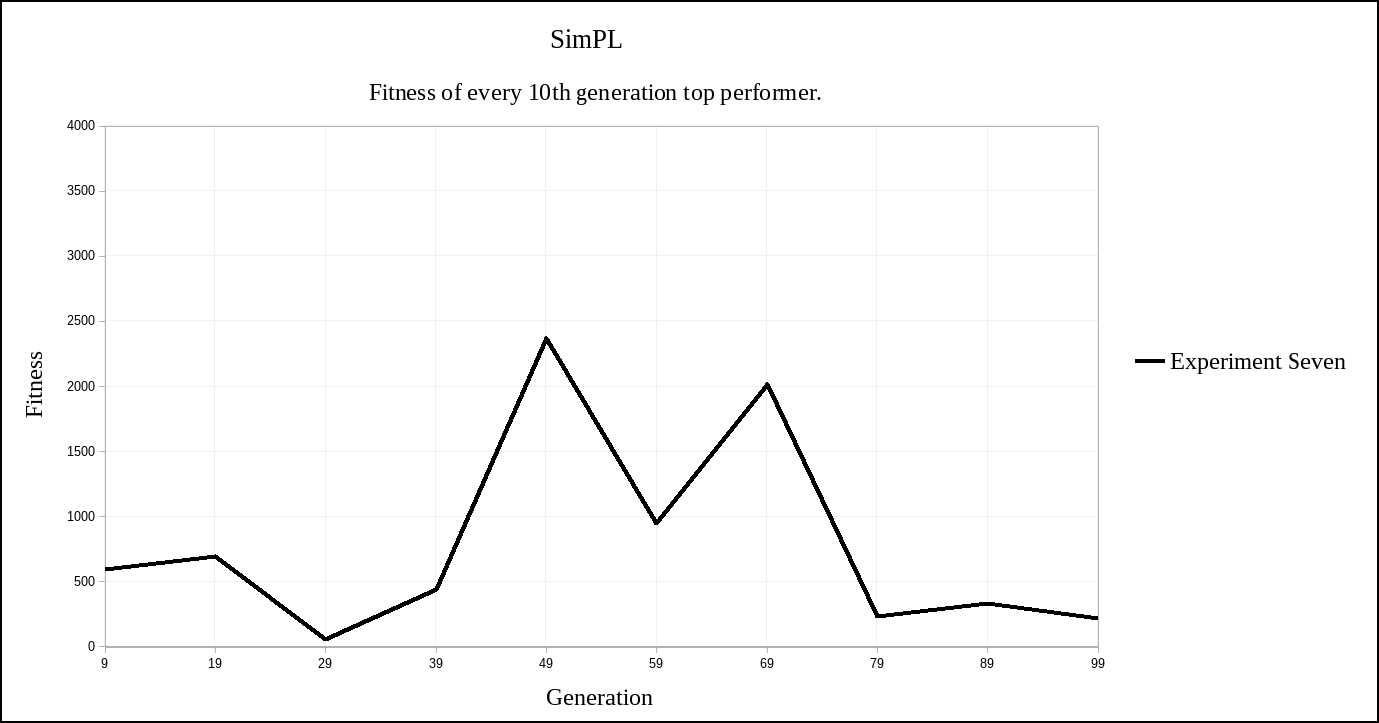
\includegraphics[width=1\textwidth]{figures/exp7_10_tops.png}
  \caption{Here you see the fitness of every 10th generation top performer for experiment seven.}
  \label{fig:exp7_10_tops}
\end{figure}

\begin{figure}[H]  
  \centering
  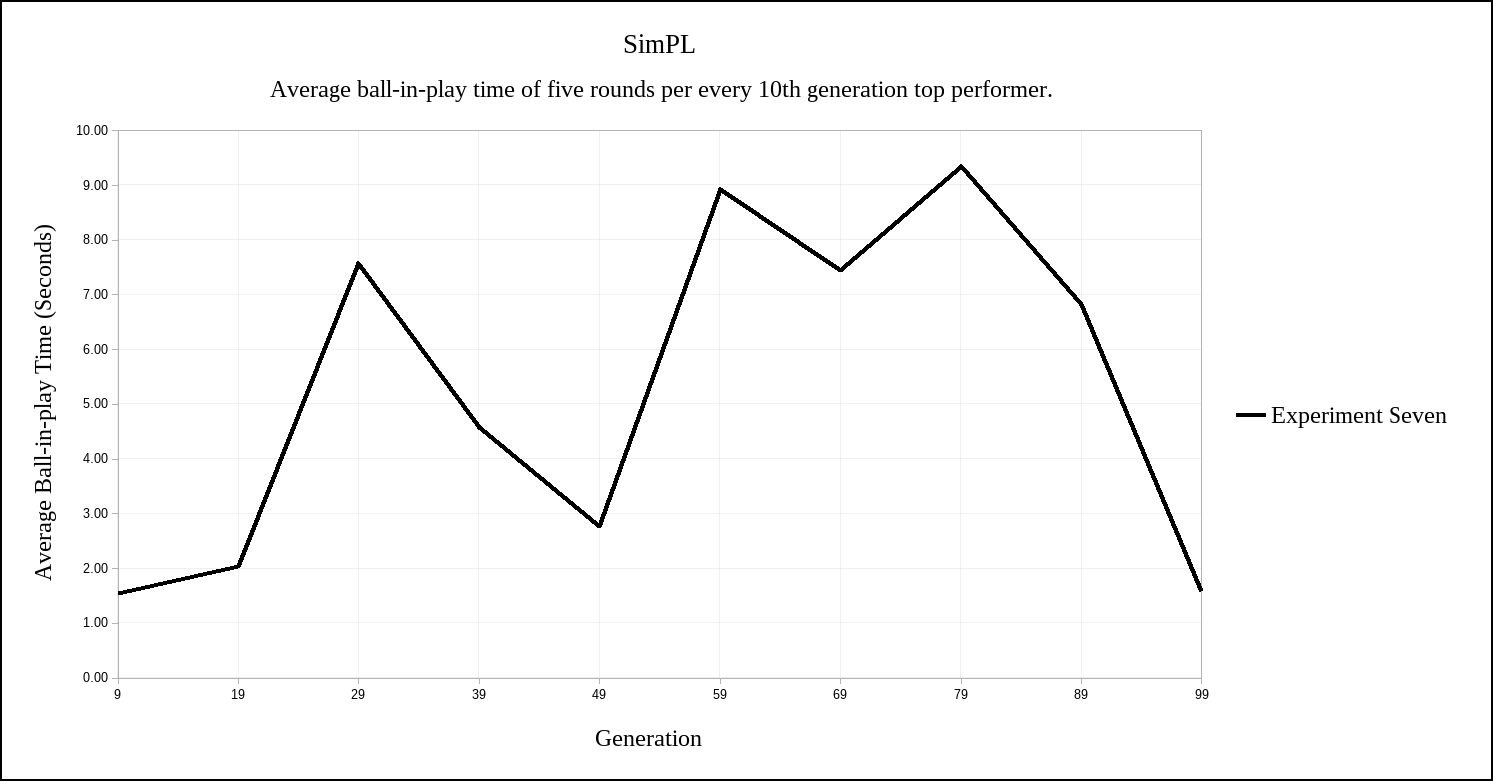
\includegraphics[width=1\textwidth]{figures/exp7_10_tops_times.png}
  \caption{Here you see the average ball-in-play time (in seconds) of five rounds per every 10th generation top performer for experiment seven.}
  \label{fig:exp7_10_tops_times}
\end{figure}

\subsection{Comparative Results}

This section illustrates comparative results by plotting all curves on the same axes (Figures \ref{fig:all_avg_fit} through \ref{fig:all_10_tops_times}).

\subsubsection{Average fitness over 100 generations.}

\begin{figure}[H]  
  \centering
  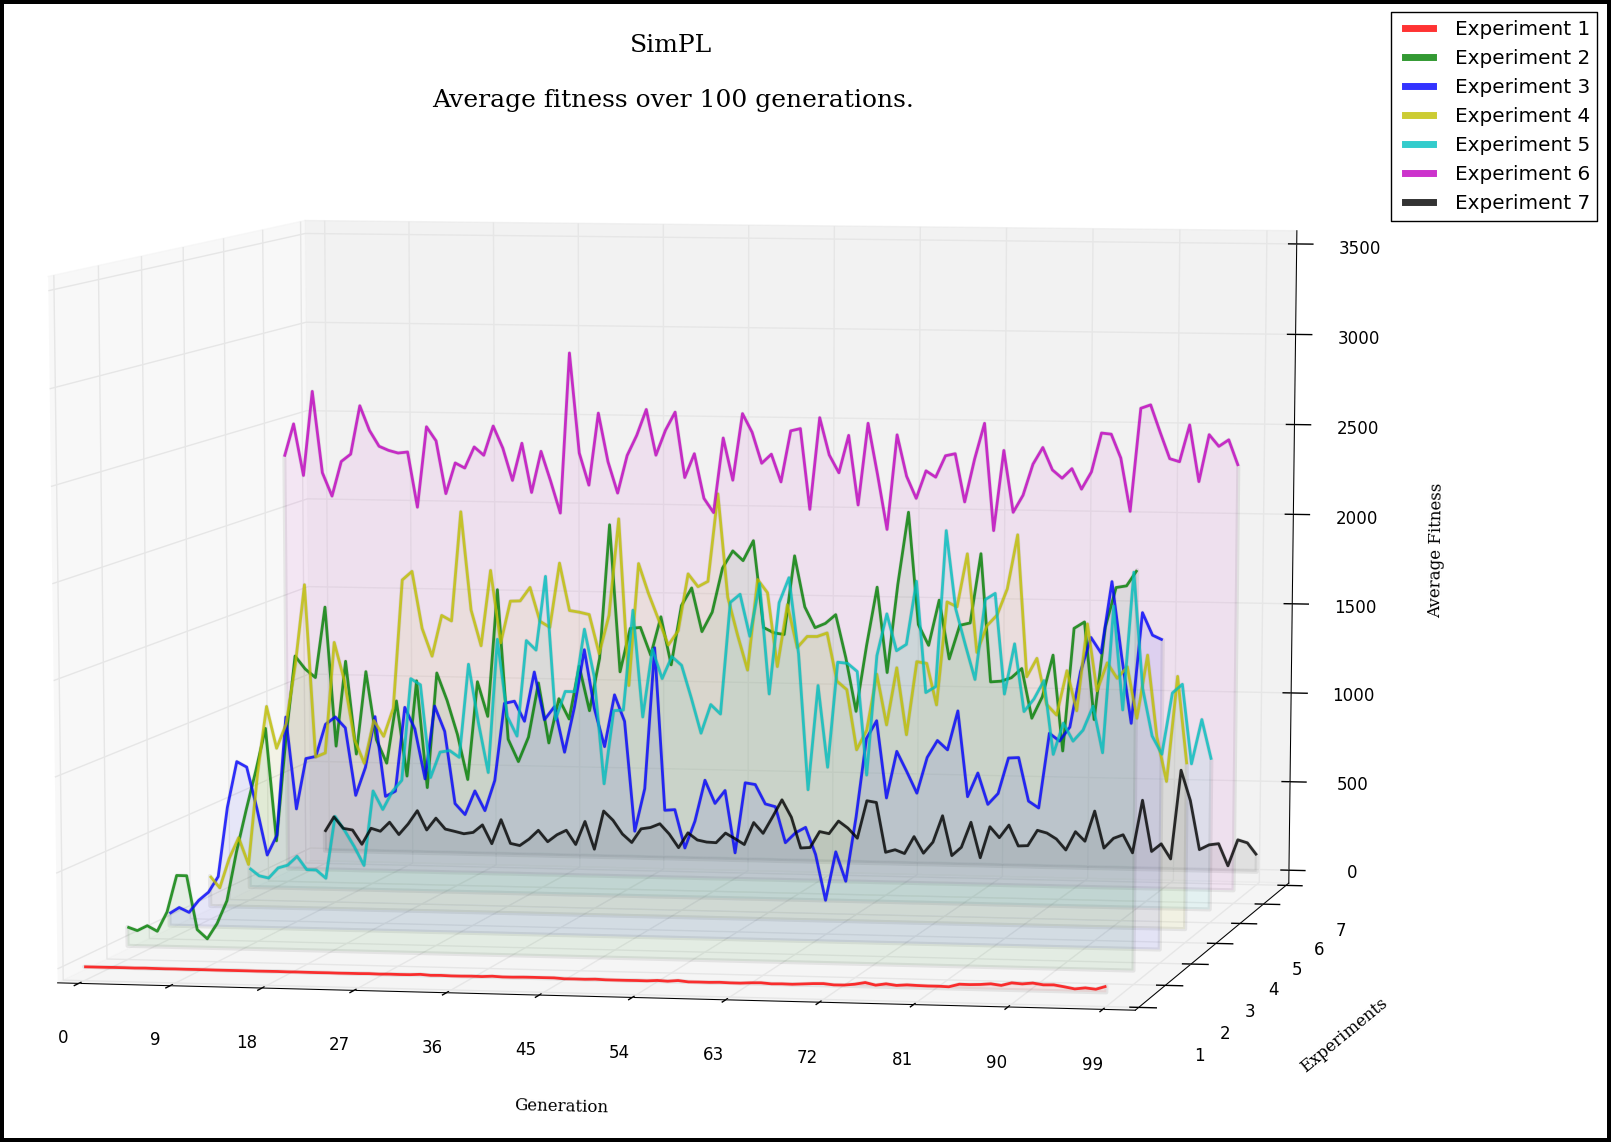
\includegraphics[width=1\textwidth]{figures/all_avg_fit.png}
  \caption{Here you see the average fitness over 100 generations for experiments one through seven.}
  \label{fig:all_avg_fit}
\end{figure}

\subsubsection{Fitness of every 10th generation top performer.}

\begin{figure}[H]  
  \centering
  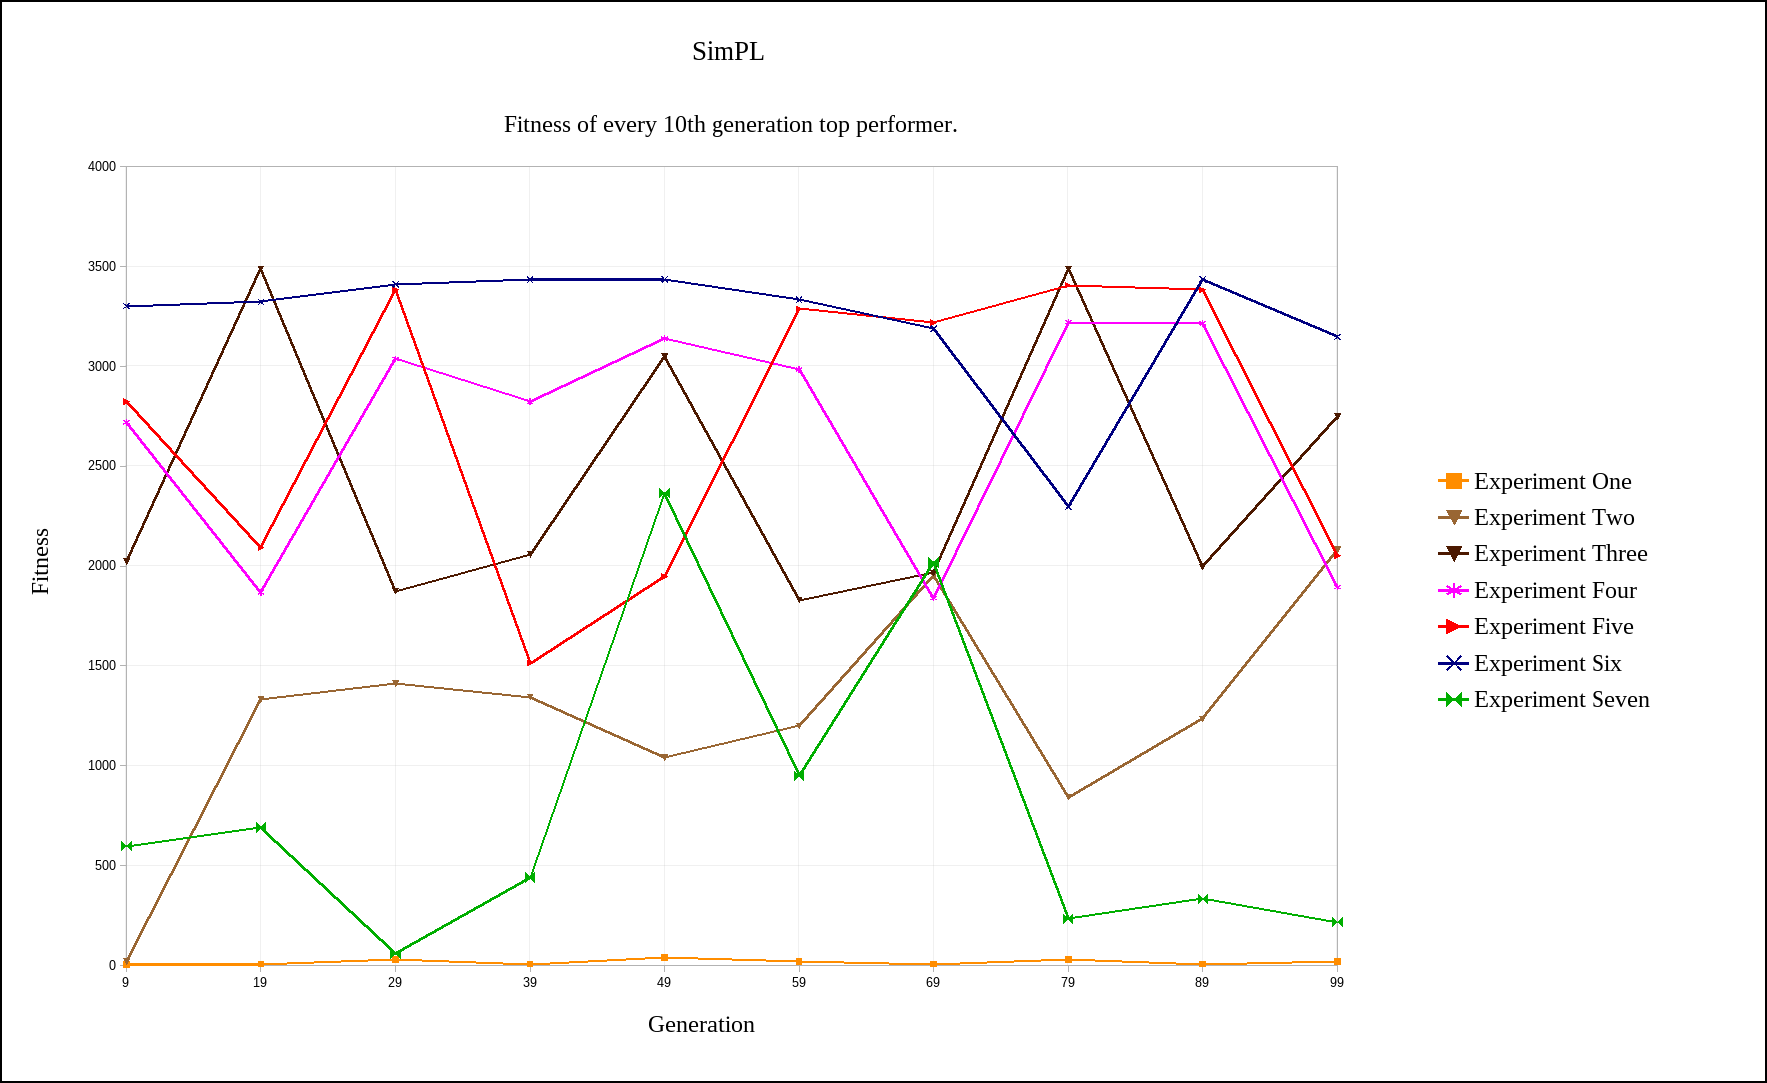
\includegraphics[width=1\textwidth]{figures/all_10_tops.png}
  \caption{Here you see the fitness of every 10th generation top performer for experiments one through seven.}
  \label{fig:all_10_tops}
\end{figure}

\subsubsection{Average ball-in-play time (in seconds) of five rounds per every 10th generation top performer.}

\begin{figure}[H]  
  \centering
  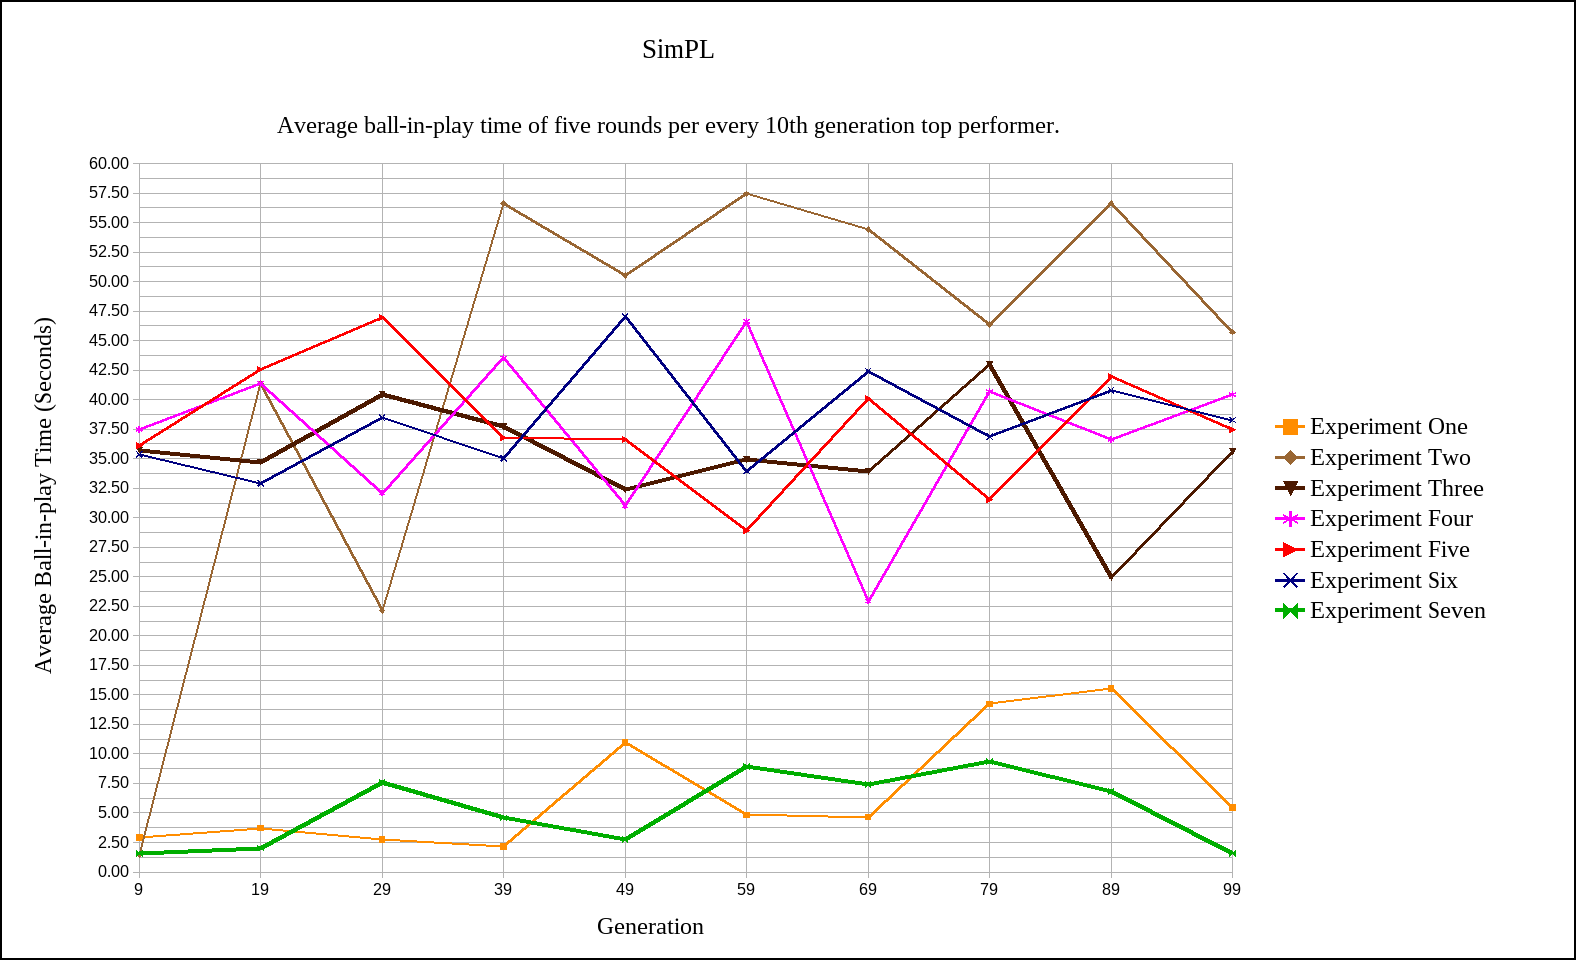
\includegraphics[width=1\textwidth]{figures/all_10_tops_times.png}
  \caption{Here you see the average ball-in-play time (in seconds) of five rounds per every 10th generation top performer for experiments one through seven.}
  \label{fig:all_10_tops_times}
\end{figure}

%\subsection{Experiment three, four, and five.}

%\begin{figure}[H]  
%  \centering
%  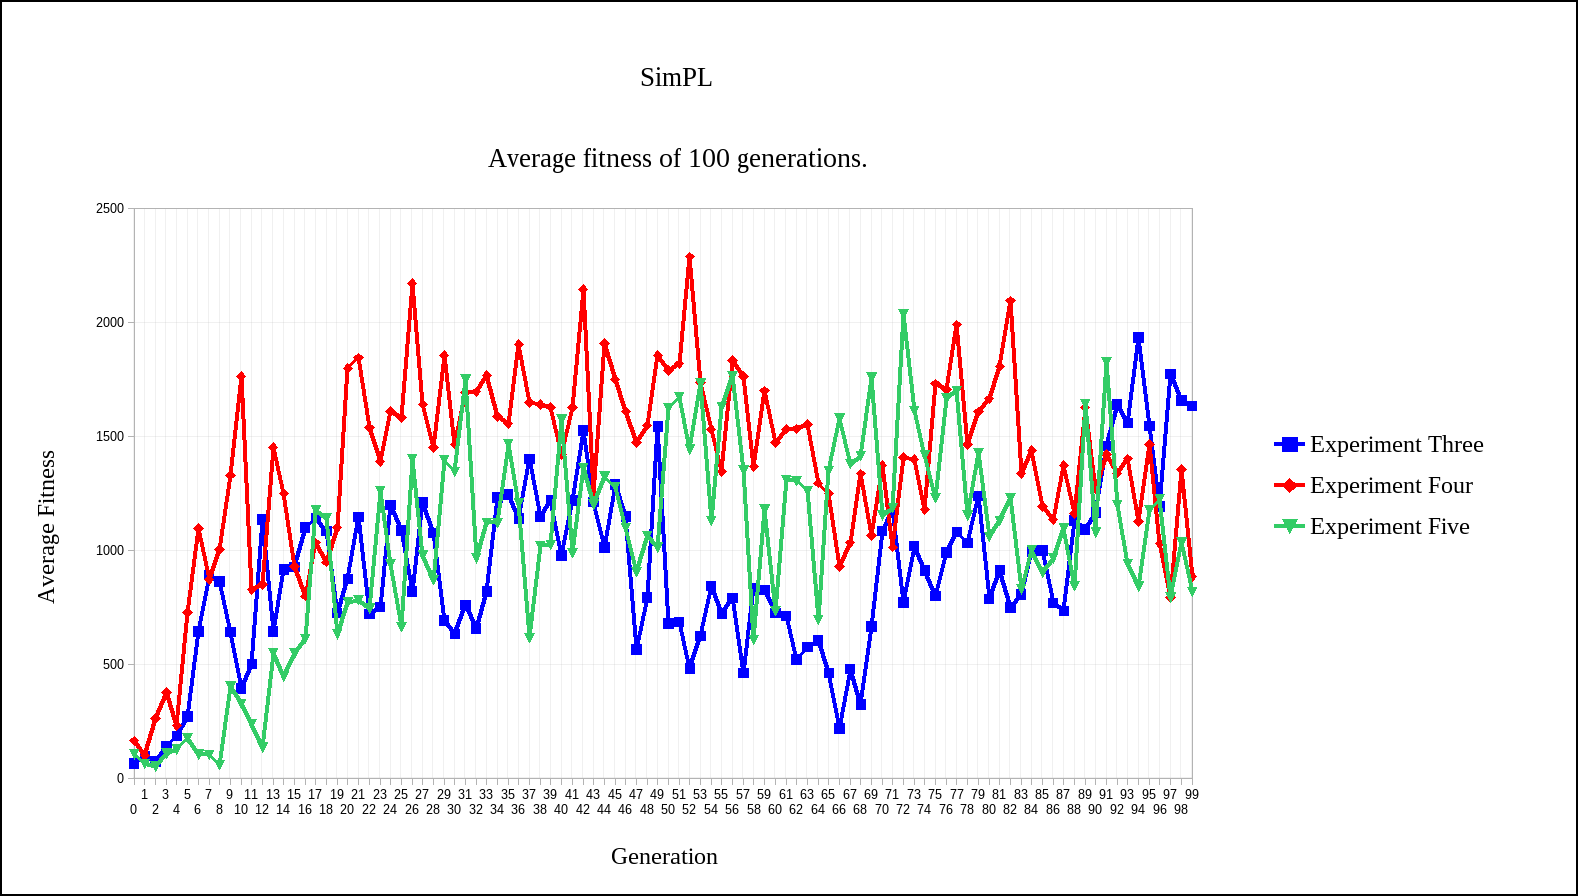
\includegraphics[width=1\textwidth]{figures/exp345_avg_fit.png}
%  \caption{Here you see the average fitness over 100 generations for experiment three, four, and five.}
%  \label{fig:exp345_avg_fit}
%\end{figure}

%\begin{figure}[H]  
%  \centering
%  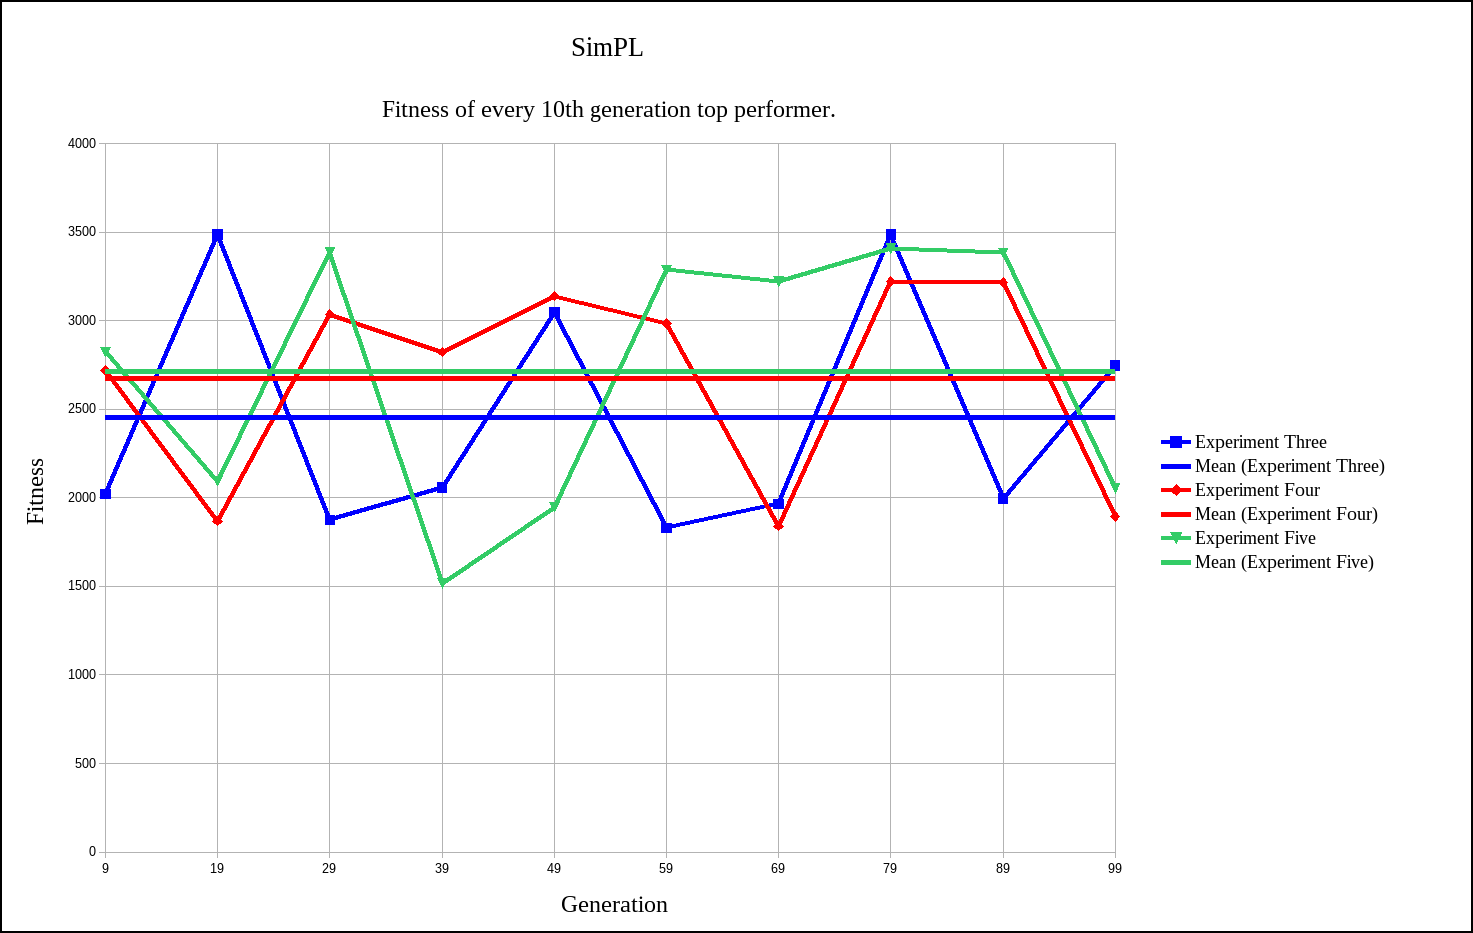
\includegraphics[width=1\textwidth]{figures/exp345_10_tops.png}
%  \caption{Here you see the fitness of the every 10th generation top performer for experiment three, four, and five.}
%  \label{fig:exp345_10_tops}
%\end{figure}

%\begin{figure}[H]  
%  \centering
%  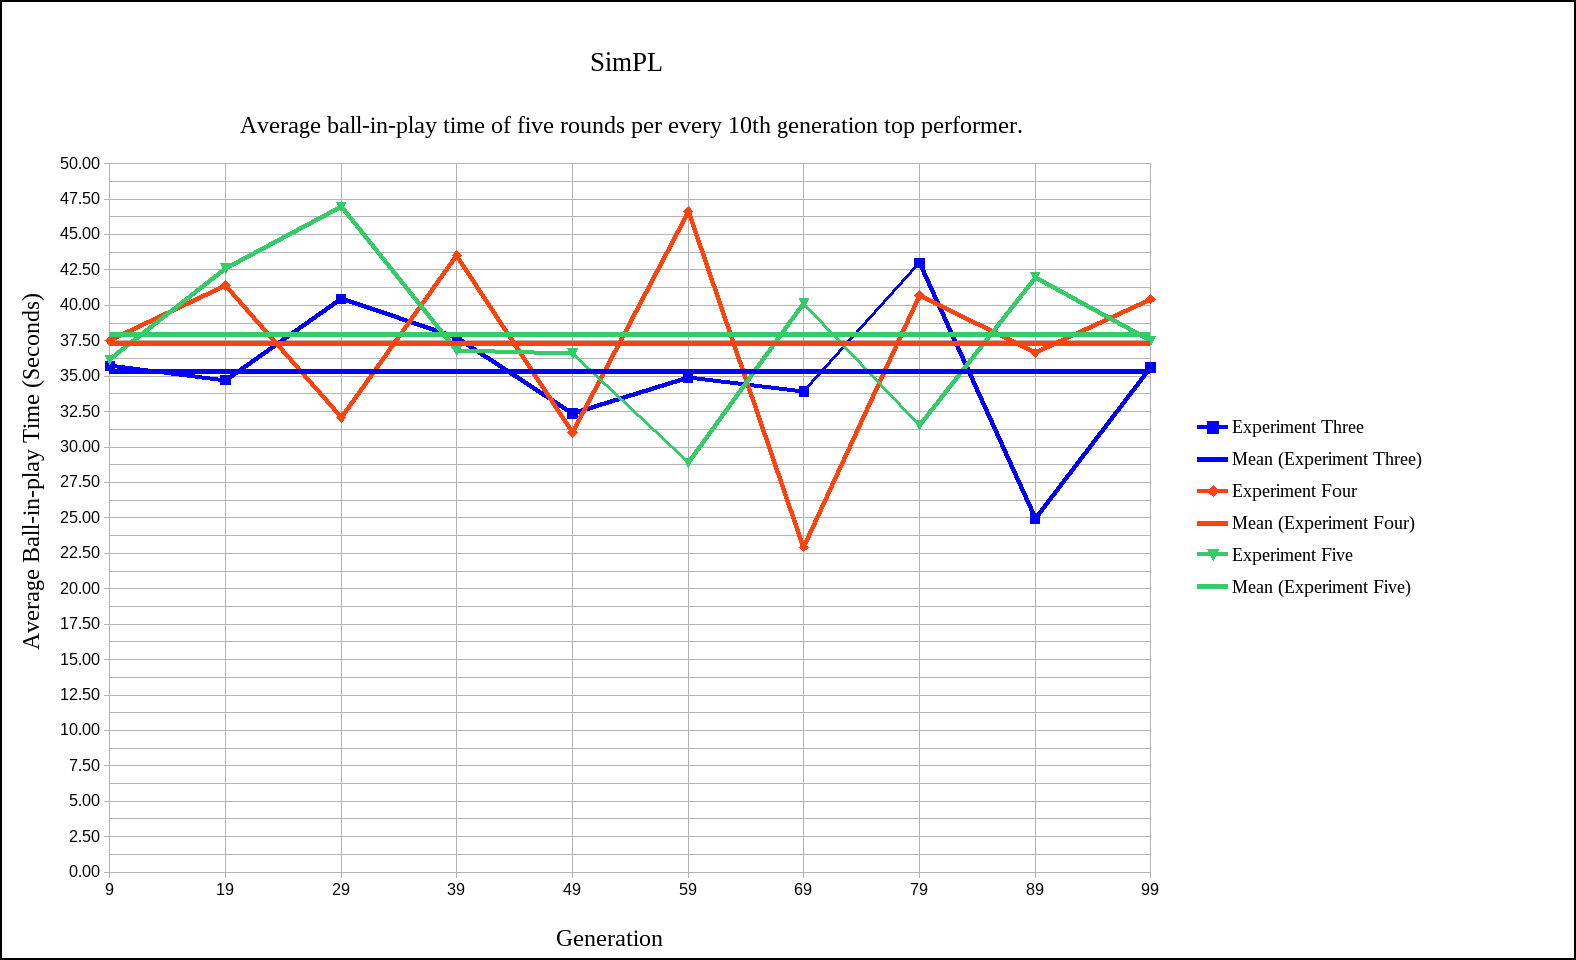
\includegraphics[width=1\textwidth]{figures/exp345_10_tops_times.png}
%  \caption{Here you see the average ball-in-play time (in seconds) of five rounds per every 10th generation top performer for experiment three, four, and five.}
%  \label{fig:exp345_10_tops_times}
%\end{figure}

%\subsection{Experiment four, five, and six.}

%\begin{figure}[H]  
%  \centering
%  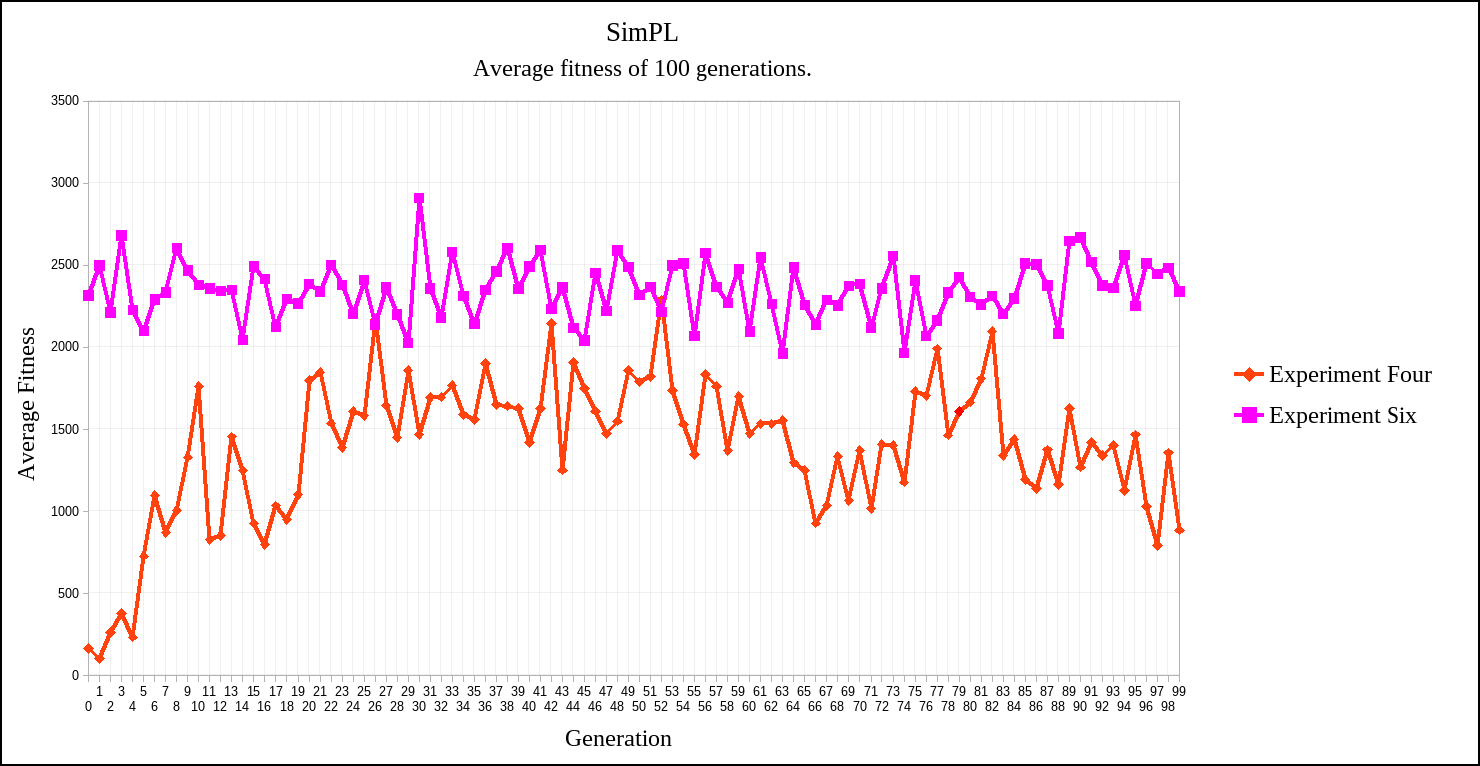
\includegraphics[width=1\textwidth]{figures/exp46_avg_fit.png}
%  \caption{Here you see the average fitness over 100 generations for experiment four and six.}
%  \label{fig:exp46_avg_fit}
%\end{figure}

%\begin{figure}[H]  
%  \centering
%  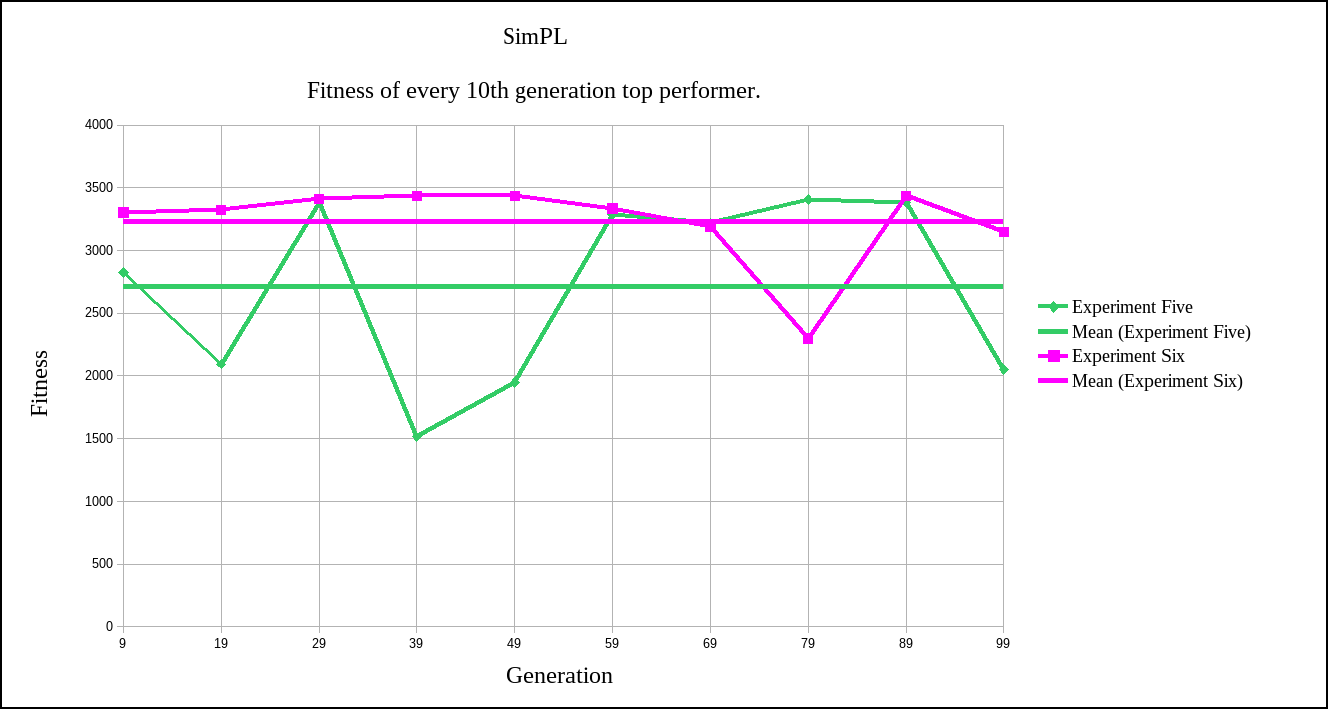
\includegraphics[width=1\textwidth]{figures/exp56_10_tops.png}
%  \caption{Here you see the fitness of the every 10th generation top performer for experiment five and six.}
%  \label{fig:exp56_10_tops}
%\end{figure}

%\begin{figure}[H]  
%  \centering
%  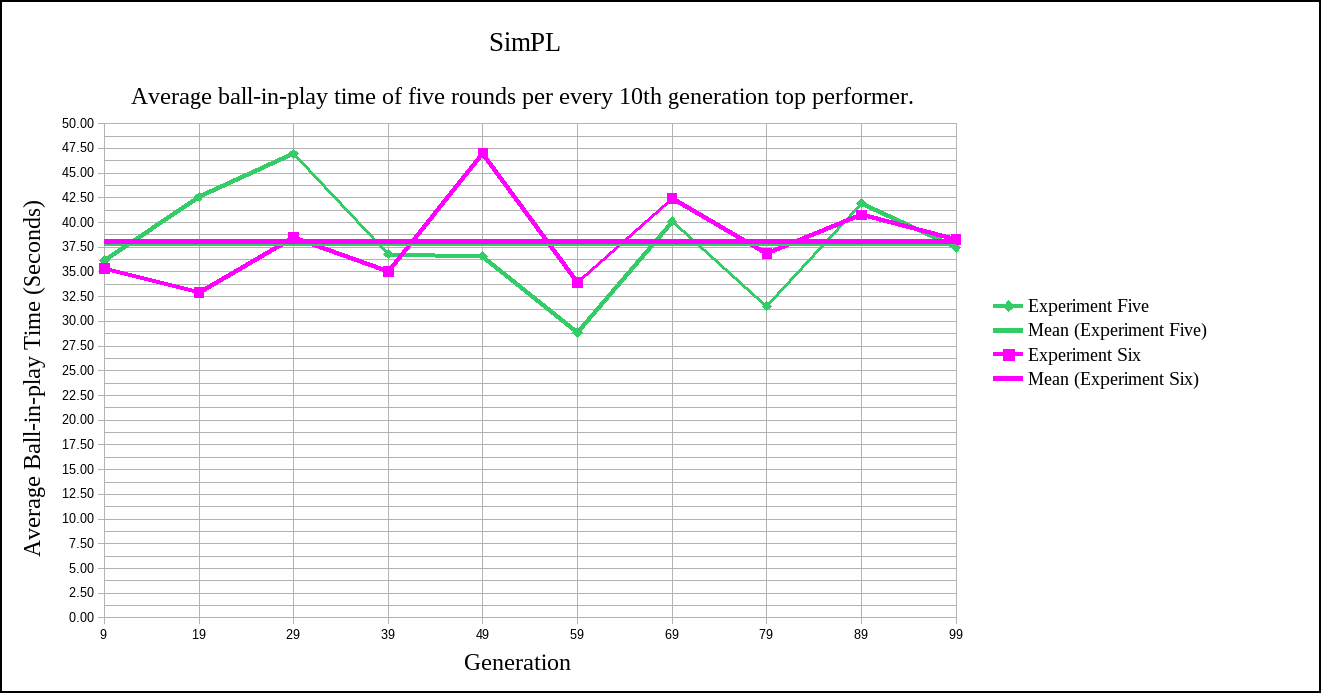
\includegraphics[width=1\textwidth]{figures/exp56_10_tops_times.png}
%  \caption{Here you see the average ball-in-play time (in seconds) of five rounds per every 10th generation top performer for experiment five and six.}
%  \label{fig:exp56_10_tops_times}
%\end{figure}

%\subsection{Experiment one, two, three, four, five, six, and seven.}

\section{Conclusion}

The genetic algorithm developed for SimPL should prove to be a robust basis for the genetic algorithm needed to solve a harder problem of tuning a 3D physics engine (project BBAutoTune). The principles and techniques of evolutionary algorithms learned during the SimPL project will certainly carry over to the more difficult project, BBAutoTune. And while the problem domain of SimPL and BBAutoTune are only somewhat similar, the problems faced and worked out during the development of SimPL should alleviate problems faced while developing BBAutoTune. As the results show, the genetic algorithm for SimPL performed well, producing neural network weight solutions that had the paddle keeping the ball in the arena for almost a minute. Had it not been for the round termination criteria of the ball's velocity magnitude dropping below $100$, most of the paddles (with high fitnesses) would have kept the ball in the arena indefinitely. Thus, the goal to learn about and to cultivate a genetic algorithm capable of tuning parameters with respect to a fitness landscape was certainly accomplished.     

\bibliographystyle{plain}
\bibliography{bibliography.bib}

\end{document}
